\documentclass[10pt]{article}

%==============================================================================
% PREAMBLE — styled after the AutoAgent technical-report format:
% blue numbered headings, rounded boxed abstract, dotted ToC leaders,
% "Figure N" captions, and full-width illustrative diagrams.
%==============================================================================
\usepackage[margin=1in]{geometry}
\usepackage{amsmath, amssymb, amsthm}
\usepackage{booktabs}
\usepackage{graphicx}
\usepackage{enumitem}
\usepackage{xcolor}
\usepackage{tikz}
\usetikzlibrary{positioning, arrows.meta, calc, shapes.misc, backgrounds, fit}
\usepackage{pgfplots}
\pgfplotsset{compat=1.18}
\usepackage[most]{tcolorbox}
\tcbuselibrary{skins}
\usepackage{titlesec}
\usepackage{tocloft}
\usepackage[labelfont=bf, labelsep=quad, font=small]{caption}

% --- Color palette (AutoAgent-style) ---
\definecolor{headblue}{RGB}{61, 107, 191}     % section headings, links
\definecolor{absbg}{RGB}{235, 242, 252}       % abstract box background
\definecolor{popblue}{RGB}{222, 235, 250}     % GAUSE panel fill
\definecolor{popblueD}{RGB}{90, 130, 200}     % GAUSE panel frame
\definecolor{reworange}{RGB}{253, 238, 222}   % reward-driven panel fill
\definecolor{reworangeD}{RGB}{226, 140, 60}   % reward-driven panel frame
\definecolor{okgreen}{RGB}{60, 145, 90}
\definecolor{badred}{RGB}{200, 60, 60}
\definecolor{dormgray}{RGB}{150, 150, 150}

\usepackage[colorlinks=true, linkcolor=headblue, citecolor=headblue,
            urlcolor=headblue]{hyperref}

% --- Blue numbered headings ---
\titleformat{\section}{\Large\bfseries\color{headblue}}{\thesection}{0.8em}{}
\titleformat{\subsection}{\large\bfseries\color{headblue}}{\thesubsection}{0.8em}{}
\titleformat{\subsubsection}{\normalsize\bfseries\color{headblue}}{\thesubsubsection}{0.8em}{}

% --- Dotted leaders in the table of contents ---
\renewcommand{\cftsecleader}{\cftdotfill{\cftdotsep}}
\renewcommand{\cftsecfont}{\normalsize}
\renewcommand{\cftsecpagefont}{\normalsize}
\setcounter{tocdepth}{2}

% --- Boxed abstract (rounded, light blue) ---
\newtcolorbox{abstractbox}{enhanced, breakable, colback=absbg, colframe=headblue!45,
  boxrule=0.6pt, arc=8pt, left=14pt, right=14pt, top=8pt, bottom=10pt}

% --- Design/recipe callout box ---
\newtcolorbox{designbox}{colback=blue!4, colframe=headblue!55, boxrule=0.5pt,
  arc=3pt, left=8pt, right=8pt, top=5pt, bottom=5pt}

\newtheorem{observation}{Observation}
\newtheorem{principle}{Principle}
\newtheorem{proposition}{Proposition}

\newcommand{\SI}{\mathrm{SI}}
\newcommand{\E}{\mathbb{E}}

% --- TikZ styles shared by the diagrams ---
\tikzset{
  panel/.style={rounded corners=4pt, draw=#1, thick, inner sep=8pt},
  blk/.style={rounded corners=2.5pt, draw=#1!70!black, fill=#1!18, thick,
              align=center, font=\footnotesize, inner sep=4pt},
  chip/.style={rounded corners=2pt, draw=#1!70!black, fill=#1!25,
               align=center, font=\scriptsize, inner sep=3pt,
               minimum width=1.35cm, minimum height=0.5cm},
  lay/.style={rounded corners=2pt, draw=#1!75!black, fill=#1!15,
              align=center, font=\scriptsize, inner sep=2.5pt,
              minimum width=3.1cm, minimum height=0.52cm},
  arr/.style={-{Stealth[length=2.4mm]}, thick},
  lbl/.style={font=\scriptsize, align=center},
}

\title{\textbf{GAUSE: Competition-Driven Specialization and\\
Reward-Independent Capacity Assignment for Learner Populations}\\[0.35cm]
\large An Explanatory Companion: Architecture, Mechanisms, Demonstrations,
and Applications}

\author{Yuhao Li\thanks{Contact: Yuhao Li (\texttt{li88@sas.upenn.edu}).}\\
University of Pennsylvania}

\date{June 2026}

\begin{document}

\maketitle
\vspace{-0.45cm}

\begin{abstractbox}
\begin{center}
{\color{headblue}\bfseries Abstract}
\end{center}
\vspace{-0.1cm}
\noindent\small
Learning systems that serve many environmental regimes with capacity-limited
learners face a persistent allocation problem: which learner handles which regime,
and---when the environment is non-stationary---who \emph{keeps} a regime that falls
dormant? We present \textbf{GAUSE} (Generalist-averse Affinity Update for Specialist
Emergence), a deliberately minimal population-learning framework with three tightly
coupled components: \emph{per-regime belief learning} (Thompson sampling over a
shared method inventory), \emph{niche-affinity tracking} (a canonical
exponentiated-gradient update on the regime simplex), and \emph{winner-take-all
competitive exclusion} (only the per-step winner reinforces its niche). At its core
is one emergent property: the converged regime-to-agent assignment is
\emph{reward-independent}, so a specialist idles while its niche is dormant and
retains its expertise. This property, not specialization per se, is what separates
mechanisms that survive non-stationarity from those that do not. Across five
capacity-allocation arms (capacity-bounded monolith, learned Mixture-of-Experts
router, fixed random niches, an EOI/CDS-style diversity objective, and emergent
competition), every reward-chasing allocation forgets dormant regimes while every
reward-independent one retains the regimes it covers---and competition secures both
at once ($\sim$70\% lower post-reactivation error than the reward-driven router,
robust to swapping hard eviction for soft interference), recovering an \emph{oracle
fixed-assignment} skyline without being handed the assignment.

The comparison above is \emph{task-incremental} (every arm sees the regime label).
Dropping the label, a class-incremental variant that infers the regime from
competence alone still retains on synthetic streams ($0.38$ post-reactivation vs.\
$1.07$ for a label-free forgetting monolith). We then test it on \emph{real} data
(UCI Gas Sensor Array Drift) and report the outcome honestly: the label-free recovery
\emph{collapses} under real feature overlap, bounding the class-incremental claim to
\emph{separable-signal} regimes; and a full-capacity online classifier does
\emph{not} catastrophically forget on these features---relocating the forgetting
story to the representation-sharing \emph{neural} regime. On real data, accordingly,
the contribution is a \emph{mechanism and lens}, not a performance win.

The remaining evidence supports that reading. Across six real-world domains
($145{,}294$ records) and synthetic tasks the framework self-organizes into
one-per-regime specialists (mean SI $=0.65$ from competition alone) and matches
purpose-built diversity and routing baselines on coverage with none of their
machinery. Four further experiments close the design space: the router's forgetting
reappears with \emph{neural experts} on two standard benchmarks (permuted-digits
$+62\%$, Split-CIFAR-100 $+22\%$); a \emph{hybrid} reservation router isolates
reward-independence of \emph{protection} as the operative property; and drift and
population-sizing sweeps map the mechanism's failure modes. We close with an
evidence-tiered survey of applications (regime-switching finance, edge sensing, and
elastic memory for agentic-AI / mixture-of-experts systems).
Code and data: \url{https://github.com/HowardLiYH/GAUSE}.
\end{abstractbox}

\vspace{0.25cm}
\noindent\textbf{Keywords:} emergent specialization; competitive exclusion;
multi-agent learning; catastrophic forgetting; mixture-of-experts;
reward-independent assignment

\newpage
\tableofcontents
\newpage

%==============================================================================
\section{Introduction}
%==============================================================================

\begin{center}
\itshape``Two species with identical ecological niches cannot stably coexist.''\\[2pt]
\normalfont ---the competitive exclusion principle \cite{gause1934struggle, hardin1960competitive}
\end{center}

Populations of learners that share an environment---trading strategies in a
market, sensors in a distributed network, experts inside a mixture-of-experts
model---face a coordination problem that single learners do not: how should the
population \emph{divide} a heterogeneous task space, without a central
coordinator, so that every regime of the environment is served by a competent
specialist? Despite decades of progress in multi-agent learning
\cite{zhang2020deep}, three intertwined limitations persist in standard
approaches.

First, \textbf{shared objectives homogenize}. Cooperative multi-agent
reinforcement learning methods (IQL \cite{tan1993multi}, VDN, QMIX
\cite{rashid2018qmix}, MAPPO \cite{yu2022surprising}) optimize a shared task
return, and a well-documented consequence is that agents converge to
near-identical policies. In our head-to-head re-runs, all four methods reach a
Specialization Index below $0.02$ on every domain---no division of labor emerges
by default. Second, \textbf{explicit coordination is expensive}. Methods that do
produce diverse roles---diversity-MARL (ROMA \cite{wang2020roma}, RODE
\cite{wang2021rode}, MAVEN \cite{mahajan2019maven}, EOI \cite{jiang2021eoi},
CDS \cite{li2021cds}), quality-diversity archives
\cite{mouret2015illuminating, pugh2016quality}, or learned gating
networks---require auxiliary machinery: intrinsic identifiability rewards,
behavior descriptors chosen \emph{a priori}, or a trained router. Each adds
objectives, hyperparameters, and failure modes of its own. Third, and least
appreciated, \textbf{reward-driven capacity allocation forgets}
\cite{french1999catastrophic, kirkpatrick2017overcoming}. When the environment
is non-stationary and per-learner capacity is bounded, any mechanism that
allocates capacity by chasing current reward---a single capacity-bounded model,
or a Mixture-of-Experts gate trained on task reward---systematically overwrites
knowledge of regimes that are currently dormant, and pays a full relearning
cost each time a regime reactivates. The dormant regime is precisely the one
emitting no reward signal, so a reward-driven allocator receives no signal to
protect it.

To address these limitations, we introduce a cohesive design philosophy centered
on a single ecological mechanism: \textbf{competitive exclusion}
\cite{gause1934struggle, hardin1960competitive, macarthur1958population}. The
framework, named \textbf{GAUSE} (Generalist-averse Affinity Update for
Specialist Emergence)\footnote{The name also honors G.~F.~Gause, whose
competitive exclusion principle (1934) the mechanism operationalizes.}, is built from three integrated
components (Figure~\ref{fig:architecture}):

\textbf{First}, each agent maintains \emph{per-regime method beliefs}---Beta
distributions over the success of each prediction method in each regime, acted
on by Thompson sampling. This is the agent's competence: what it knows how to do,
and where. \textbf{Second}, each agent tracks a \emph{niche affinity}
distribution over regimes, updated by the canonical exponentiated-gradient
(Hedge / multiplicative-weights) rule
\cite{kivinen1997exponentiated, freund1997decision, arora2012multiplicative}.
This is the agent's identity: where it
belongs. \textbf{Third}, agents are coupled solely through \emph{winner-take-all
competition}: at each step, all agents act, and only the best performer
reinforces its affinity for the current regime. No communication, no shared
reward, no gate, no diversity objective. Competition makes homogeneous strategies
unstable---identical agents split the same wins, so deviating to a less-contested
regime pays---and the population partitions into one-per-regime specialists.

The key insight of this document is that the resulting assignment has a property
that purpose-built alternatives lack: \emph{it is reward-independent at
convergence}. A converged specialist holds its niche by identity, not by
moment-to-moment reward, so when its regime goes dormant the specialist simply
idles and \emph{retains} its expertise (Figure~\ref{fig:timeline}). We formalize
this as a
\textbf{reward-independence principle} (Section~\ref{sec:principle}), show that
it cleanly dichotomizes five capacity-allocation mechanisms in controlled
experiments (every reward-chasing arm forgets; every reward-independent arm
retains), and demonstrate that it independently corroborates recent
mixture-of-experts theory \cite{li2024moecl}, which finds that the gating
network's updates must be \emph{terminated} for continual-learning convergence.

In summary, this work makes the following key contributions:

\textbf{1) Catastrophic forgetting reframed as a signal-availability problem.}
Our most portable contribution is a lens, not an algorithm. Under bounded capacity,
the quantity that most needs protecting---a dormant regime's knowledge---is exactly
the one emitting no reward, so the protective signal is structurally correlated with
the activity signal. Any allocator that protects capacity using current reward is
therefore \emph{blind} to dormant regimes by construction. We turn this observation
into a scoped \textbf{reward-independence principle}
(Principle~\ref{prin:ria}): within the class of mechanisms whose only protection is
the assignment itself, reward-independence is \emph{necessary} for retention, and
reward-independence \emph{plus persistent coverage} is \emph{sufficient}. We verify
the prediction across five allocation mechanisms, confirm it transfers to
\emph{gradient-trained neural experts} on two standard continual-learning benchmarks
(permuted-digits and Split-CIFAR-100; the failure is architecture-agnostic and
benchmark-portable), bound it with a real-data reality check
(Section~\ref{sec:realdata}: on near-separable real features a full-capacity learner
does \emph{not} forget, localizing the forgetting claim to the representation-sharing
regime), and stress-test it with a \emph{hybrid} reward-driven router carrying an
explicit reservation term, which retains exactly when its protection becomes
reward-independent. The GAUSE algorithm is then one
instantiation that reaches a reward-independent, fully-covering assignment
\emph{for free}, where prior art needs a hand-tuned freeze schedule or an auxiliary
diversity reward.

\textbf{2) A coordination-free specialization mechanism.} GAUSE couples
winner-take-all competition with an exponentiated-gradient niche update and
nothing else. Competition alone (niche bonus $\lambda=0$) drives mean SI to
$0.65$ across six real domains; with the default bonus the population reaches
SI $\approx 0.99$ and one-per-regime coverage.

\textbf{3) Honest benchmarking against purpose-built baselines.} Rather than
compare only to cooperative MARL (which does not try to specialize), we compare
to an EOI/CDS-style learned-diversity objective, a learned MoE router, and a
hybrid router with a memory-preservation term, all at matched capacity. Spatial
coverage proves to be a commodity all arms achieve; competition's value there is
parsimony. Retention is not a commodity: the reward-driven router fails it
decisively, in both tabular and gradient-trained form.

\textbf{4) A meaningfulness audit.} We show that the Specialization Index
certifies \emph{organization}, not exploitable structure (it is invariant to
regime-label shuffling and inflatable by the learning rate), and we localize
exactly when division of labor improves task accuracy---under bounded capacity
and non-stationarity---and when it does not. The audit extends to the mechanism's
own failure modes: under \emph{intra-regime drift} the converged assignment pins
stale specialists (worse than a relearning monolith) until a staleness trigger
re-opens competition, and scarce populations ($N<R$) under-cover regardless of
per-agent capacity.

\textbf{5) Matching the oracle ceiling without the assignment.} Since every arm is
handed the regime label, the honest competitor is an \emph{oracle fixed assignment}
given both the labels and a perfect covering permutation---the retention skyline. We
show GAUSE recovers it without being handed the assignment: within $0.030$ of the
floor at $K{=}1$ and statistically indistinguishable for $K\ge3$, and
indistinguishable at \emph{every} $K$ under the soft memory model. Competition's
value is automatic, pre-commitment-free recovery of the oracle partition, not
beating it.

\textbf{6) The retention result survives dropping the label (class-incremental).}
All of the above is task-incremental (the regime label is given). We then remove it:
a variant that infers the active regime from competence alone still self-organizes
against the \emph{hidden} regimes (SI $0.75$, coverage $0.86$) and retains
($0.38$ post-reactivation vs.\ $1.07$ for a label-free forgetting monolith),
detecting reactivation purely from input similarity. On \emph{real}, feature-rich
data with genuine overlap (UCI gas sensor; Section~\ref{sec:realdata}), however,
this label-free recovery \emph{collapses} (post-reactivation $\to 0$, and the
dissociation against the label-free monolith vanishes). We therefore report the
class-incremental result honestly as a proof of concept bounded to
\emph{separable-signal} regimes---demonstrated where a separating signal exists, not
a general capability.

%==============================================================================
\section{Related Work}
%==============================================================================

We review prior work along five dimensions closely related to GAUSE.

\textbf{Cooperative MARL.} Independent Q-Learning \cite{tan1993multi},
value-decomposition methods (VDN, QMIX \cite{rashid2018qmix}), and multi-agent
policy gradients (MAPPO \cite{yu2022surprising}) optimize shared objectives
with centralized training. These methods are the right baselines for cooperative
control, but they do not attempt diversity, and empirically they homogenize: in
our re-runs all reach SI $\le 0.02$. We treat them as confirmatory contrast, not
as competitors on specialization.

\textbf{Diversity- and role-emergence MARL.} ROMA \cite{wang2020roma} and RODE
\cite{wang2021rode} learn role embeddings; MAVEN \cite{mahajan2019maven}
injects diverse exploration; EOI \cite{jiang2021eoi} and CDS \cite{li2021cds}
add intrinsic individuality or mutual-information objectives; R3DM
\cite{goel2025r3dm} discovers roles through dynamics models. These methods do
produce division of labor, at the cost of explicit diversity machinery. We
benchmark directly against an EOI/CDS-style intrinsic-reward arm and find it a
strong baseline: it matches competition on coverage for $K\ge2$ and retains
dormant regimes (its assignment is driven by an identity reward, not task
reward---the reward-independence principle again). Competition's advantage over
it is parsimony, not dominance.

\textbf{Quality-diversity optimization.} MAP-Elites
\cite{mouret2015illuminating} and novelty search \cite{lehman2011evolving}
maintain archives of diverse high performers, but require behavior descriptors
defined \emph{a priori}. GAUSE needs no descriptors: niches are
discovered by the dynamics.

\textbf{Mixture-of-experts in continual learning.} Recent theory
\cite{li2024moecl} establishes that MoE can mitigate catastrophic forgetting
\cite{french1999catastrophic, parisi2019continual} by isolating tasks in
experts---\emph{provided} experts are plentiful relative to tasks and the gating
network's updates are eventually terminated, without which continual task
arrival destabilizes routing. Our experiments occupy exactly the regime those
provisos exclude (fixed total capacity, experts forced into reuse, gate still
learning) and show that isolation then breaks down: the router inherits the
monolith's forgetting. Freezing the gate is, in our terms, making the assignment
reward-independent; competition reaches that state emergently, with no freezing
schedule to tune.

\textbf{Ecological niche theory.} The competitive exclusion principle
\cite{gause1934struggle, hardin1960competitive} and MacArthur's resource
partitioning \cite{macarthur1958population} describe how competition alone
drives species into complementary niches \cite{grant2014finches}.
GAUSE operationalizes this for artificial learners and inherits its
most useful property: the partition, once formed, is maintained by identity
rather than by ongoing payoff, which is what makes it robust to dormancy.

%==============================================================================
\section{The GAUSE Framework: A Unified Architecture for
Emergent Division of Labor}
%==============================================================================

This section presents the integrated architecture. We first articulate the
design philosophy (3.1), then detail the architectural blueprint (3.2), and
finally explain the per-step dynamics that realize self-organization (3.3).
Figure~\ref{fig:architecture} contrasts the standard reward-driven allocation
stack with the GAUSE architecture.

% ---------------------------------------------------------------- FIGURE 1 ---
\begin{figure}[t]
\centering
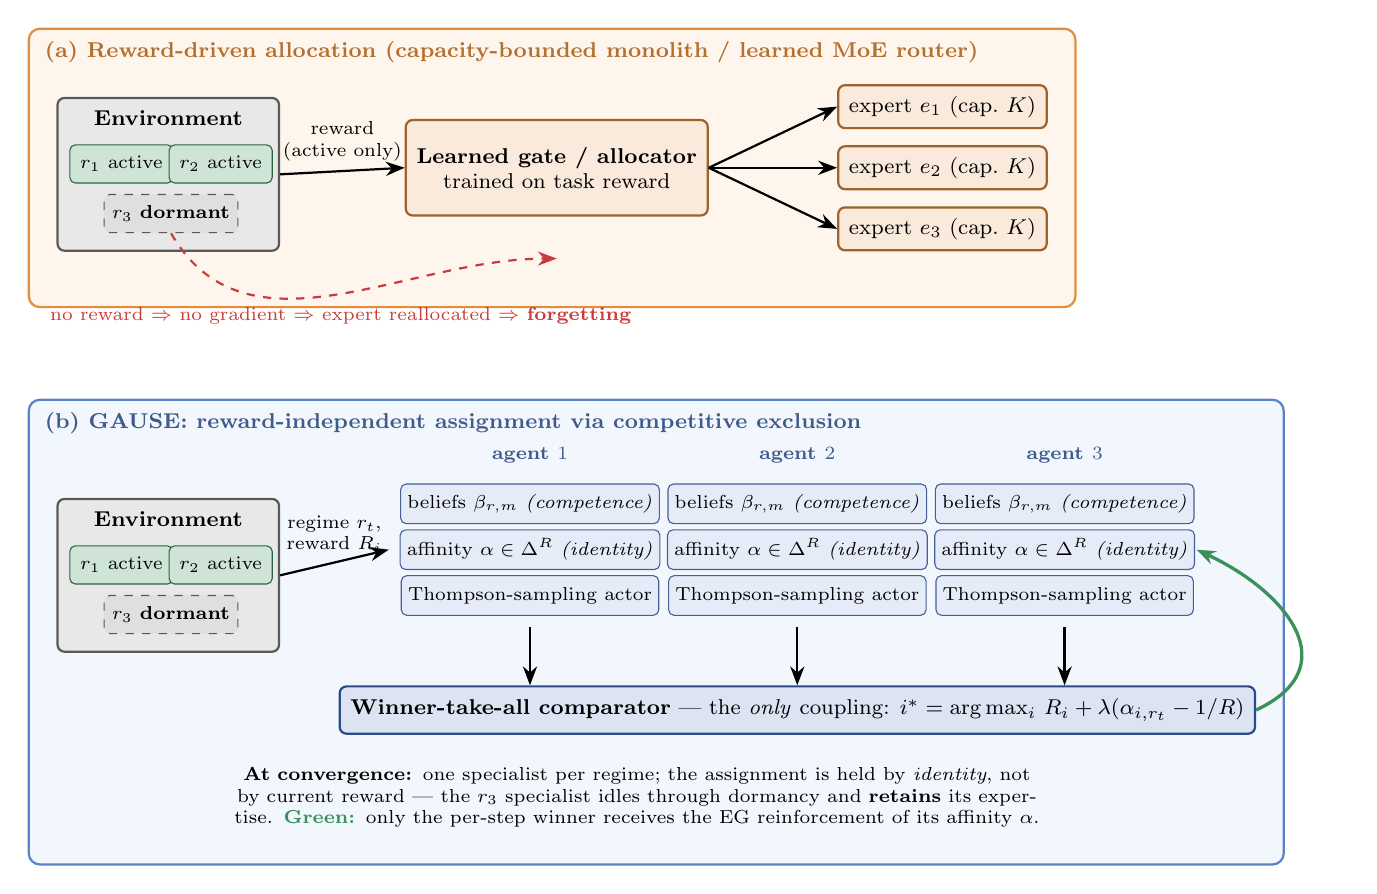
\begin{tikzpicture}[scale=0.97, every node/.style={transform shape}]

% ===================== PANEL (a): reward-driven allocation ==================
\begin{scope}[yshift=0cm]
  % environment
  \node[blk=gray, minimum width=2.9cm, minimum height=2.0cm, anchor=south west]
    (envA) at (0,0.25) {};
  \node[font=\footnotesize\bfseries, anchor=north] at ($(envA.north)+(0,-0.06)$)
    {Environment};
  \node[chip=okgreen] (ra1) at ($(envA.south west)+(0.85,1.15)$) {$r_1$ active};
  \node[chip=okgreen] (ra2) at ($(envA.south west)+(2.15,1.15)$) {$r_2$ active};
  \node[chip=gray, dashed] (ra3) at ($(envA.south west)+(1.5,0.5)$)
    {$r_3$ \textbf{dormant}};

  % gate
  \node[blk=reworangeD, minimum width=3.0cm, minimum height=1.25cm]
    (gate) at (6.55,1.35) {\textbf{Learned gate / allocator}\\
                           trained on task reward};

  % experts
  \node[blk=reworangeD, minimum width=2.2cm] (e1) at (11.6,2.15)
    {expert $e_1$ (cap.\ $K$)};
  \node[blk=reworangeD, minimum width=2.2cm] (e2) at (11.6,1.35)
    {expert $e_2$ (cap.\ $K$)};
  \node[blk=reworangeD, minimum width=2.2cm] (e3) at (11.6,0.55)
    {expert $e_3$ (cap.\ $K$)};

  % arrows
  \draw[arr] (envA.east) -- node[lbl, above]{reward\\(active only)} (gate.west);
  \draw[arr] (gate.east) -- (e1.west);
  \draw[arr] (gate.east) -- (e2.west);
  \draw[arr] (gate.east) -- (e3.west);

  % failure annotation
  \draw[arr, badred, dashed] (ra3.south) to[out=-60, in=180]
    node[lbl, below, text=badred, xshift=2pt, yshift=-1pt]
    {no reward $\Rightarrow$ no gradient $\Rightarrow$ expert reallocated
     $\Rightarrow$ \textbf{forgetting}} ($(gate.south)+(0,-0.55)$);

  % panel frame
  \begin{scope}[on background layer]
    \node[panel=reworangeD, fill=reworange!55, fit=(envA)(gate)(e1)(e3),
          inner xsep=10pt, inner ysep=20pt] (panelA) {};
  \end{scope}
  \node[anchor=north west, font=\footnotesize\bfseries, text=reworangeD!80!black]
    at ($(panelA.north west)+(0.1,-0.06)$)
    {(a) Reward-driven allocation (capacity-bounded monolith / learned MoE router)};
\end{scope}

% ===================== PANEL (b): GAUSE ============================
\begin{scope}[yshift=-5.6cm]
  % environment
  \node[blk=gray, minimum width=2.9cm, minimum height=2.0cm, anchor=south west]
    (envB) at (0,0.6) {};
  \node[font=\footnotesize\bfseries, anchor=north] at ($(envB.north)+(0,-0.06)$)
    {Environment};
  \node[chip=okgreen] (rb1) at ($(envB.south west)+(0.85,1.15)$) {$r_1$ active};
  \node[chip=okgreen] (rb2) at ($(envB.south west)+(2.15,1.15)$) {$r_2$ active};
  \node[chip=gray, dashed] (rb3) at ($(envB.south west)+(1.5,0.5)$)
    {$r_3$ \textbf{dormant}};

  % agent cards
  \foreach \i/\x in {1/6.2, 2/9.7, 3/13.2} {
    \node[lay=popblueD] (bel\i) at (\x, 2.55)
      {beliefs $\beta_{r,m}$ \emph{(competence)}};
    \node[lay=popblueD] (aff\i) at (\x, 1.95)
      {affinity $\alpha \in \Delta^{R}$ \emph{(identity)}};
    \node[lay=popblueD] (act\i) at (\x, 1.35)
      {Thompson-sampling actor};
    \begin{scope}[on background layer]
      \node[panel=popblueD, fill=popblue!70, inner sep=3.5pt,
            fit=(bel\i)(aff\i)(act\i)] (agent\i) {};
    \end{scope}
    \node[anchor=south, font=\scriptsize\bfseries, text=popblueD!70!black]
      at (agent\i.north) {agent $\i$};
  }

  % winner-take-all bar
  \node[blk=headblue, minimum width=10.4cm, minimum height=0.62cm]
    (wta) at (9.7, -0.15)
    {\textbf{Winner-take-all comparator} --- the \emph{only} coupling:
     $i^{*} = \arg\max_i\, R_i + \lambda(\alpha_{i,r_t} - 1/R)$};

  % arrows: env -> agents
  \draw[arr] (envB.east) -- node[lbl, above]{regime $r_t$,\\reward $R_i$}
    (agent1.west);
  % agents -> wta
  \draw[arr] (agent1.south) -- (wta.north -| agent1.south);
  \draw[arr] (agent2.south) -- (wta.north -| agent2.south);
  \draw[arr] (agent3.south) -- (wta.north -| agent3.south);
  % winner reinforcement: return arrow along the right edge (explained in note)
  \draw[arr, okgreen, very thick]
    (wta.east) to[out=25, in=-25, looseness=1.5] ($(aff3.east)+(0.02,0)$);

  % converged note
  \node[lbl, text width=13.6cm, anchor=north] (convnote) at (7.6, -0.78)
    {\textbf{At convergence:} one specialist per regime; the assignment is held
     by \emph{identity}, not by current reward --- the $r_3$ specialist idles
     through dormancy and \textbf{retains} its expertise.
     \textcolor{okgreen}{\textbf{Green:}} only the per-step winner receives the
     EG reinforcement of its affinity $\alpha$.};

  % panel frame (topPad reserves room for the panel title above the agent labels)
  \coordinate (topPad) at (9.7, 3.55);
  \begin{scope}[on background layer]
    \node[panel=popblueD, fill=popblue!40,
          fit=(envB)(agent3)(wta)(convnote)(topPad),
          inner ysep=10pt, inner xsep=10pt] (panelB) {};
  \end{scope}
  \node[anchor=north west, font=\footnotesize\bfseries, text=popblueD!70!black]
    at ($(panelB.north west)+(0.1,-0.06)$)
    {(b) GAUSE: reward-independent assignment via competitive exclusion};
\end{scope}

\end{tikzpicture}
\caption{The GAUSE architecture, contrasted with reward-driven
allocation. \textbf{(a)} A gate (or a single bounded model) assigns capacity by
chasing current task reward; a dormant regime emits no reward gradient, so its
capacity is silently reallocated and must be relearned on reactivation.
\textbf{(b)} GAUSE couples agents only through per-step
winner-take-all competition; each agent's niche affinity $\alpha$ concentrates
on the regime it wins, and the converged one-per-regime partition is
\emph{structural}---it persists with no reward flow, which is the source of the
retention results in Section~\ref{sec:experiments}.}
\label{fig:architecture}
\end{figure}

\subsection{Design Philosophy: The Competitive-Exclusion Loop}

Contemporary approaches to division of labor treat the assignment of learners to
tasks as something to be \emph{optimized}: a gate is trained, a diversity
objective is added, roles are learned. GAUSE is founded on the opposite
principle: \textbf{the assignment should be an equilibrium, not an objective}.
We formalize this as the competitive-exclusion loop, a recursive paradigm
structured around four functions (Figure~\ref{fig:loop}):

\begin{designbox}
\textbf{Compete}: all agents act on the current regime; one wins.\\
\textbf{Reinforce}: only the winner strengthens its affinity for that regime.\\
\textbf{Differentiate}: losers' relative affinities drift toward less-contested
regimes.\\
\textbf{Stabilize}: once each agent owns a regime, deviation is unprofitable;
the partition is a fixed point.
\end{designbox}

% ---------------------------------------------------------------- FIGURE 2 ---
\begin{figure}[t]
\centering
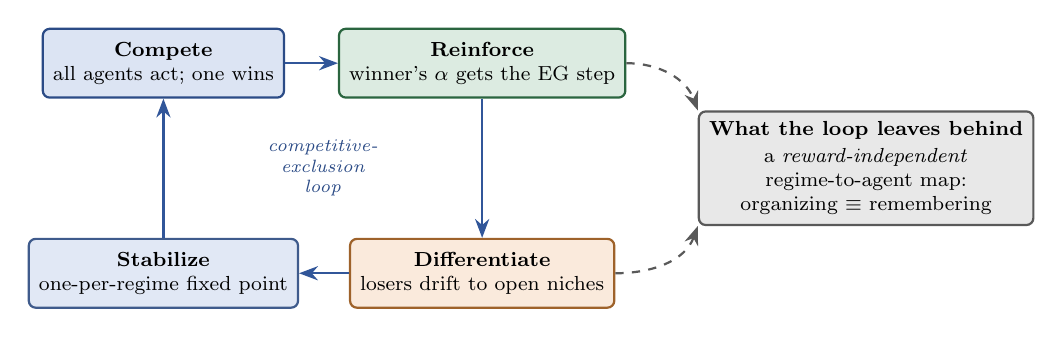
\begin{tikzpicture}[scale=0.92, every node/.style={transform shape}]
  \def\rx{4.4} \def\ry{1.45}
  \node[blk=headblue, minimum width=3.2cm, minimum height=0.95cm] (compete)
    at (0, \ry) {\textbf{Compete}\\all agents act; one wins};
  \node[blk=okgreen, minimum width=3.2cm, minimum height=0.95cm] (reinforce)
    at (\rx, \ry) {\textbf{Reinforce}\\winner's $\alpha$ gets the EG step};
  \node[blk=reworangeD, minimum width=3.2cm, minimum height=0.95cm] (diff)
    at (\rx, -\ry) {\textbf{Differentiate}\\losers drift to open niches};
  \node[blk=popblueD, minimum width=3.2cm, minimum height=0.95cm] (stab)
    at (0, -\ry) {\textbf{Stabilize}\\one-per-regime fixed point};

  \draw[arr, headblue!80!black] (compete.east) -- (reinforce.west);
  \draw[arr, headblue!80!black] (reinforce.south) -- (diff.north);
  \draw[arr, headblue!80!black] (diff.west) -- (stab.east);
  \draw[arr, headblue!80!black] (stab.north) -- (compete.south);

  \node[lbl, text=headblue!70!black, font=\scriptsize\itshape, align=center]
    at (\rx/2, 0)
    {competitive-\\exclusion\\loop};

  % what the loop leaves behind
  \node[blk=gray, minimum width=4.1cm, minimum height=1.5cm, align=center]
    (legacy) at (9.7, 0)
    {\textbf{What the loop leaves behind}\\[1pt]
     a \emph{reward-independent}\\regime-to-agent map:\\
     organizing $\equiv$ remembering};
  \draw[arr, dashed, gray!70!black] (reinforce.east) to[out=0, in=110]
    (legacy.north west);
  \draw[arr, dashed, gray!70!black] (diff.east) to[out=0, in=-110]
    (legacy.south west);
\end{tikzpicture}
\caption{The competitive-exclusion loop. Compete--Reinforce--Differentiate
iterates until Stabilize: each agent owns a regime and deviation is
unprofitable. The loop's by-product is its most valuable output---a converged
assignment that no longer depends on the flow of reward.}
\label{fig:loop}
\end{figure}

The key property of this loop is \emph{what it leaves behind}. Because the
converged partition is a fixed point of identity (each agent's affinity
concentrates on its niche), it no longer depends on the flow of reward. An agent
whose niche is dormant receives no wins, but it also receives no pressure to
abandon its niche---it simply idles. This is the structural source of the
retention results in Section~\ref{sec:experiments}: the loop intrinsically
unifies \emph{organizing} with \emph{remembering}.

\subsection{Architectural Blueprint: Components and Their Roles}

The loop is instantiated through three principal components per agent, plus one
population-level rule (Figure~\ref{fig:architecture}b).

\textbf{1. Method-Belief Store: The Competence Layer.} Each agent $i$ maintains,
for each regime $r$ it has encountered, a Beta distribution
$\mathrm{Beta}(\beta^{+}_{i,r,m},\, \beta^{-}_{i,r,m})$ over the success rate of
each method $m$ in a shared inventory of $M$ methods. This store answers
\emph{``what works here?''} and is updated by standard Bayesian counting. In the
bounded-capacity experiments the store is explicitly finite: it holds at most
$K$ regimes, with either least-recently-used eviction (hard model) or graded
interference decay (soft model)---Section~\ref{sec:capacity}.

\textbf{2. Niche Affinity: The Identity Layer.} Each agent maintains a
distribution $\alpha_i \in \Delta^R$ over regimes---its evolving answer to
\emph{``where do I belong?''} Affinity is updated only on wins, by the canonical
exponentiated-gradient rule (Section~\ref{sec:affinity}), and read out through
the Specialization Index $\SI(\alpha) = 1 - H(\alpha)/\log R$, which is $1$ for
a one-hot specialist and $0$ for a uniform generalist.

\textbf{3. Thompson-Sampling Actor: The Decision Layer.} At each step the agent
samples $\tilde{\theta}_m \sim \mathrm{Beta}(\beta^{+},\beta^{-})$ for every
method and plays the argmax---a principled exploration--exploitation balance
requiring no tuned exploration schedule.

\textbf{4. Winner-Take-All Rule: The Population Coupling.} The \emph{only}
interaction between agents is the per-step competition: the agent with the
highest (optionally niche-shaped) reward is declared winner and is the only one
to reinforce its affinity. There is no communication channel, no shared critic,
no gate, and no diversity term. This minimality is deliberate: every emergent
property of the system must be attributable to competition, because nothing else
couples the agents.

\subsection{System Dynamics: One Step of the Loop}

The components interact in a fast per-step cycle. Given the environment in
regime $r_t$:

\begin{enumerate}[itemsep=2pt]
    \item \textbf{Act.} Every agent $i$ selects a method $m_i$ by Thompson
    sampling from its beliefs for $r_t$ (agents without competence in $r_t$ act
    uninformed) and receives raw reward $R_i$.
    \item \textbf{Score.} Each agent's competitive score adds an additive niche
    bonus centred on the uniform affinity:
    $\tilde{R}_i = R_i + \lambda\,(\alpha_{i,r_t} - 1/R)$, with $\lambda \ge 0$.
    At $\lambda = 0$ the bonus vanishes and raw reward decides.
    \item \textbf{Select winner.} $i^* = \arg\max_i \tilde{R}_i$.
    \item \textbf{Update beliefs.} Agents update their Beta counts for the
    methods they played (success/failure), within their capacity budget.
    \item \textbf{Update identity.} Only the winner applies the
    exponentiated-gradient affinity update for $r_t$ and renormalizes.
\end{enumerate}

Two timescales emerge from this single cycle without being designed in: a
\emph{fast} competence dynamic (beliefs sharpen within a regime in tens of
steps) and a \emph{slow} identity dynamic (affinities concentrate over hundreds
of steps). The slow dynamic is the one with the architectural consequence: once
identities have concentrated, the regime-to-agent map is fixed and
reward-independent, and the population behaves as a distributed, persistent
memory over the regime space.

%==============================================================================
\section{Niche Affinity and the Exponentiated-Gradient Update}
\label{sec:affinity}
%==============================================================================

\subsection{The Update Rule}

When agent $i$ wins in regime $r$ with normalized reward (quality) $q \in [0,1]$,
its affinity updates multiplicatively and renormalizes:
\begin{equation}
    \alpha_{i,r} \leftarrow \frac{\alpha_{i,r}\, e^{\eta q}}
    {\sum_{r'} \alpha_{i,r'}\, e^{\eta q\,\mathbf{1}[r'=r]}},
\end{equation}
the canonical exponentiated-gradient / Hedge / multiplicative-weights step on
the regime simplex \cite{kivinen1997exponentiated, freund1997decision,
arora2012multiplicative, cesa2006prediction}. Three properties motivate this
choice over additive
heuristics. \textbf{(i) Simplex preservation by construction:} affinities remain
a probability distribution with no clamping (an earlier additive variant of this
project required an undocumented clamp whose pathology suppressed roughly half
the specialization signal; replacing it with EG is what separates the current
V4 results from the V3 ones). \textbf{(ii) A constant effective rate:} the
multiplicative step does not slow down or speed up depending on the current
state in the way the clamped additive rule did. \textbf{(iii) A standard form:}
EG on the simplex is the textbook update for tracking the best coordinate,
making the algorithm's one learnable dynamic maximally legible. We deliberately
do \emph{not} claim Hedge's adversarial regret bound transfers to our coupled
winner-take-all setting; that would require separate analysis.

\subsection{Worked Demonstration}

Consider $R=3$ regimes, $\eta = 0.6$, and an agent at uniform affinity
$\alpha = (0.333, 0.333, 0.333)$. The agent wins three consecutive steps in
regime $1$ with quality $q = 1$:
\[
(0.333,0.333,0.333) \;\to\; (0.477,0.262,0.262) \;\to\; (0.624,0.188,0.188)
\;\to\; (0.751,0.124,0.124).
\]
Three wins move SI from $0$ to $0.33$; ten wins take it past $0.95$
(Figure~\ref{fig:egdemo}). The same
trajectory in reverse never occurs spontaneously: losing in regime 1 does not
push the agent away (losers do not update); it is \emph{winning elsewhere} that
re-anchors identity. This asymmetry---identity moves only on positive evidence
of fit---is what makes converged identities stable through dormancy.

% ---------------------------------------------------------------- FIGURE 3 ---
\begin{figure}[t]
\centering
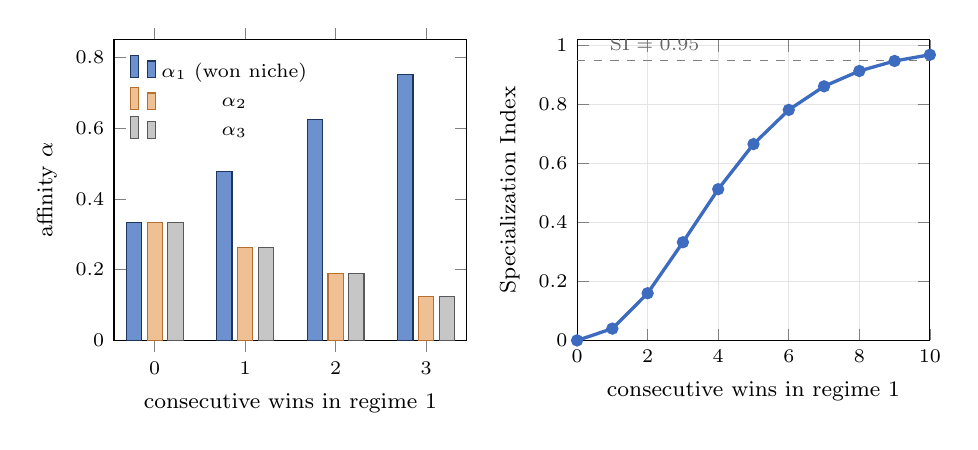
\begin{tikzpicture}
\begin{axis}[
  name=bars,
  width=0.5\textwidth, height=5.4cm,
  ybar, bar width=5.5pt,
  xlabel={consecutive wins in regime 1},
  ylabel={affinity $\alpha$},
  xtick={0,1,2,3}, ymin=0, ymax=0.85,
  legend style={font=\scriptsize, at={(0.02,0.97)}, anchor=north west,
                draw=none, fill=none},
  tick label style={font=\scriptsize},
  label style={font=\footnotesize},
  enlarge x limits=0.15,
]
\addplot[fill=headblue!75, draw=headblue!50!black]
  coordinates {(0,0.333) (1,0.477) (2,0.624) (3,0.751)};
\addplot[fill=reworangeD!55, draw=reworangeD!80!black]
  coordinates {(0,0.333) (1,0.262) (2,0.188) (3,0.124)};
\addplot[fill=gray!45, draw=gray!70!black]
  coordinates {(0,0.333) (1,0.262) (2,0.188) (3,0.124)};
\legend{$\alpha_1$ (won niche), $\alpha_2$, $\alpha_3$}
\end{axis}
\begin{axis}[
  at={($(bars.east)+(1.4cm,0)$)}, anchor=west,
  width=0.5\textwidth, height=5.4cm,
  xlabel={consecutive wins in regime 1},
  ylabel={Specialization Index},
  xmin=0, xmax=10, ymin=0, ymax=1.02,
  grid=major, grid style={gray!20},
  tick label style={font=\scriptsize},
  label style={font=\footnotesize},
]
\addplot[headblue, very thick, mark=*, mark size=1.6pt]
  coordinates {(0,0.000) (1,0.040) (2,0.160) (3,0.333) (4,0.513) (5,0.666)
               (6,0.782) (7,0.862) (8,0.914) (9,0.948) (10,0.969)};
\addplot[gray, dashed, domain=0:10] {0.95}
  node[pos=0.22, above, font=\scriptsize, text=gray!80!black]
  {$\SI = 0.95$};
\end{axis}
\end{tikzpicture}
\caption{Worked demonstration of the exponentiated-gradient affinity update
($R=3$, $\eta=0.6$, quality $q=1$). \textbf{Left:} the winning regime's
affinity grows multiplicatively while the others shrink by renormalization.
\textbf{Right:} the Specialization Index $\SI = 1 - H(\alpha)/\log R$ traced
over ten consecutive wins---identity concentrates quickly, and only positive
evidence (winning) ever moves it.}
\label{fig:egdemo}
\end{figure}

\subsection{Heterogeneous Initialization and Symmetry Breaking}

Agents start near-uniform with small random perturbations. The perturbation
carries no labels and no assignment; it only breaks ties so that the first few
competitions are not decided by coin flips alone. The eventual one-per-regime
partition is an equilibrium selected by the dynamics, not an initialization
artifact: random-shuffle controls confirm the same partition statistics under
re-drawn perturbations.

%==============================================================================
\section{Competitive Exclusion and Winner-Take-All Dynamics}
%==============================================================================

\subsection{Why Strictness Matters}

Winner-take-all is not a simplification of softer competition---it is the key
structural driver of differentiation. Under proportional (softmax) credit,
identical agents can persist indefinitely: each receives a share of every
regime's reward, and hedging across niches is stable. Under winner-take-all,
identical agents split wins evenly in expectation, so each one's per-regime
reinforcement halves; an agent that deviates to an uncontested regime wins that
regime \emph{outright}. Formally (companion paper \cite{li2026emergent},
Proposition 1), homogeneous
strategy profiles are not Nash equilibria of the winner-take-all game: a
unilateral deviation to a less-contested niche strictly increases expected
reinforcement.

\subsection{The Niche Bonus Is an Accelerator, Not the Cause}

The additive shaping term $\lambda(\alpha_{i,r_t} - 1/R)$ advantages an agent
competing in a regime it already prefers. Setting $\lambda = 0$ removes it
entirely---and specialization still emerges, with mean SI $0.65$ across the six
real domains (every domain $> 0.49$, versus $0.13$ for a random baseline). The
$\lambda$-sweep is flat and high ($\SI > 0.98$) across $\lambda \in [0.2,0.4]$
and declines at $0.5$, where over-locked winners stop contesting secondary
regimes and leave some niches under-filled. The mechanism therefore needs no
shaping to work; shaping only sharpens it.

\subsection{What the Population Looks Like After Convergence}

On every real domain, the converged population is a clean partition: each agent
holds a primary niche with affinity $\ge 0.95$, every regime is owned by at
least one agent, and the population collectively uses $86\%$ of the shared
method inventory (specialists adopt the methods suited to their niche). The
assignments are interpretable by inspection---a property no deep MARL baseline
in our comparison offers.

%==============================================================================
\section{Bounded Capacity and Memory Models}
\label{sec:capacity}
%==============================================================================

Specialization only matters when no single learner can do everything. We model
this with an explicit per-agent capacity $K$: each agent can hold beliefs for at
most $K$ of the $R$ regimes. Two memory models implement the constraint.

\subsection{Hard Model: LRU Slots}

The belief store holds $K$ regime entries; learning an uncached regime evicts
the least-recently-used entry. Eviction is total: the evicted regime's beliefs
reset to the uninformed prior, and re-encountering it costs a full relearning
period. This is the cleanest possible model of ``capacity binds.''

\subsection{Soft Model: Interference Decay}

A natural objection is that real learners do not evict discretely---knowledge
\emph{interferes} \cite{french1999catastrophic}. The soft model removes
eviction entirely: every learning
update on the active regime decays the pseudo-counts of the agent's other held
regimes by a factor that grows with how far the agent's learned footprint
exceeds $K$. Dormant regimes are never refreshed, so they decay smoothly toward
the prior---the interference account of catastrophic forgetting, with graded
rather than all-or-nothing loss. Every retention result in
Section~\ref{sec:experiments} is reproduced under both models; the headline
separation is a property of \emph{who gets updated}, not of how forgetting is
discretized.

\subsection{The Five Capacity-Allocation Arms}

All experiments compare five mechanisms at matched per-agent capacity $K$,
together with one privileged \emph{oracle skyline} (arm 6) that we use as an
upper reference rather than as a competing mechanism:

\begin{enumerate}[itemsep=2pt]
    \item \textbf{Monolith}: one agent with capacity $K$ serves everything.
    Allocation chases the active regime by necessity.
    \item \textbf{MoE router}: $N$ capacity-$K$ experts behind a learned gate
    ($\epsilon$-greedy routing; gate trained on routed-expert quality).
    Allocation chases current reward by design.
    \item \textbf{Random diversity}: $N$ agents with fixed, random capacity-$K$
    niches. Allocation is frozen---fully reward-independent, but coverage is
    accidental.
    \item \textbf{Learned diversity (EOI/CDS-style)}: all agents receive an
    intrinsic identifiability reward $\log p(i \mid r)$ on top of task quality
    \cite{jiang2021eoi, li2021cds};
    the identified owner learns the regime. Allocation follows an
    \emph{identity} signal, not task reward.
    \item \textbf{GAUSE (ours)}: winner-take-all competition;
    allocation is an emergent, converged identity.
    \item \textbf{Oracle fixed assignment (skyline)}: $N{=}R$ agents pinned to a
    hand-designed \emph{covering} assignment---at $K{=}1$ the identity permutation
    (agent $i \mapsto$ regime $i$), with no learning of \emph{where} to specialize.
    This arm is reward-independent and perfectly covering \emph{by construction} and
    pays zero discovery cost, so it marks the best achievable retention; it is
    privileged because it is handed both the regime labels and the assignment.
\end{enumerate}

This five-arm design is deliberate: the arms differ in \emph{what signal drives
capacity assignment}, which is exactly the axis the next section's principle
predicts should matter. The oracle skyline adds the natural sixth question---if
the labels are known, why not simply hand-assign?---which we answer directly in
Section~\ref{sec:principle} and Table~\ref{tab:retention}.

\paragraph{What each arm observes (and why the comparison is fair).} All six
arms receive the same information at each step: the current regime label $r_t$
and the per-method quality signal. This is the \emph{task-incremental} continual-learning
setting (task identity known), not the harder \emph{class-incremental} one (task
identity must be inferred). We make this explicit because it bounds the claim and
keeps the comparison information-symmetric: the dissociation below is \emph{not} an
artifact of GAUSE seeing the regime while the router must infer it---the MoE gate,
the monolith, and every other arm are handed exactly the same $r_t$. What differs
across arms is solely \emph{what each does with that label}: whether the
capacity assignment it induces chases current reward or is reward-independent.
GAUSE's contribution is therefore scoped precisely: \emph{given} task identity, a
self-organized reward-independent assignment retains where reward-chasing ones
forget. Removing the oracle label---inferring $r_t$ from the competence beliefs
themselves, which already form a per-regime likelihood---is the natural next step
and we return to it in Section~\ref{sec:conclusion}.

%==============================================================================
\section{The Reward-Independence Principle}
\label{sec:principle}
%==============================================================================

\subsection{Why a Reward-Driven Router Forgets}

Consider a regime $r$ that goes dormant for an extended interval while an expert
$e$ holding $r$ receives $D$ learning updates from other, active regimes.
Figure~\ref{fig:timeline} illustrates the mechanism.

\begin{observation}[Dormant regimes receive no protective signal]
\label{obs}
Under the hard capacity model, $e$ retains $r$ only if fewer than $K$ distinct
regimes are used during the interval; under the soft model, $r$'s retained
strength decays as $(1-\rho)^D \to 0$. Crucially, a dormant regime emits no
steps and hence no reward gradient: the gate update
$\Delta\,\mathrm{gate}[r][e] \propto (q_e - \tfrac12)$ is identically zero
throughout dormancy, so the router receives no signal that would lead it to
reserve $e$ for $r$. Reactivation therefore incurs the full relearning cost with
probability $\to 1$ as dormancy grows.
\end{observation}

% ---------------------------------------------------------------- FIGURE 4 ---
\begin{figure}[t]
\centering
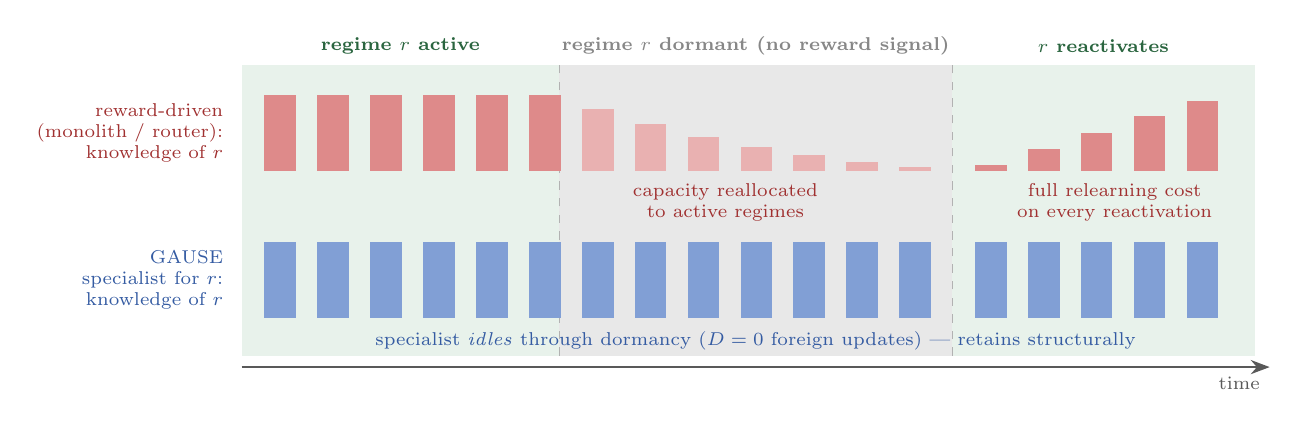
\begin{tikzpicture}[scale=0.96, every node/.style={transform shape}]
  % time axis
  \draw[arr, gray!70!black] (0,-0.4) -- (13.6,-0.4)
    node[below left, font=\scriptsize]{time};

  % phase bands
  \fill[okgreen!12] (0,-0.25) rectangle (4.2,3.6);
  \fill[gray!18]    (4.2,-0.25) rectangle (9.4,3.6);
  \fill[okgreen!12] (9.4,-0.25) rectangle (13.4,3.6);
  \node[font=\scriptsize\bfseries, text=okgreen!70!black] at (2.1,3.85)
    {regime $r$ active};
  \node[font=\scriptsize\bfseries, text=dormgray!90!black] at (6.8,3.85)
    {regime $r$ \textbf{dormant} (no reward signal)};
  \node[font=\scriptsize\bfseries, text=okgreen!70!black] at (11.4,3.85)
    {$r$ reactivates};
  \draw[dashed, gray!60] (4.2,-0.25) -- (4.2,3.6);
  \draw[dashed, gray!60] (9.4,-0.25) -- (9.4,3.6);

  % ---- row 1: reward-driven ----
  \node[font=\scriptsize, anchor=east, align=right, text=badred!80!black]
    at (-0.12, 2.7) {reward-driven\\(monolith / router):\\knowledge of $r$};
  % active: full bars
  \foreach \x in {0.3, 1.0, 1.7, 2.4, 3.1, 3.8}
    \fill[badred!60] (\x, 2.2) rectangle (\x+0.42, 3.2);
  % dormant: decaying bars
  \foreach \x/\h in {4.5/0.82, 5.2/0.62, 5.9/0.45, 6.6/0.31, 7.3/0.20,
                     8.0/0.11, 8.7/0.05}
    \fill[badred!40] (\x, 2.2) rectangle (\x+0.42, 2.2+\h);
  % reactivation: relearn from near zero
  \foreach \x/\h in {9.7/0.08, 10.4/0.28, 11.1/0.50, 11.8/0.72, 12.5/0.92}
    \fill[badred!60] (\x, 2.2) rectangle (\x+0.42, 2.2+\h);
  \node[lbl, text=badred!80!black, align=center] at (11.55, 1.78)
    {full relearning cost\\on every reactivation};
  \node[lbl, text=badred!80!black, align=center] at (6.4, 1.78)
    {capacity reallocated\\to active regimes};

  % ---- row 2: GAUSE ----
  \node[font=\scriptsize, anchor=east, align=right, text=headblue!85!black]
    at (-0.12, 0.75) {GAUSE\\specialist for $r$:\\knowledge of $r$};
  \foreach \x in {0.3, 1.0, 1.7, 2.4, 3.1, 3.8, 4.5, 5.2, 5.9, 6.6, 7.3,
                  8.0, 8.7, 9.7, 10.4, 11.1, 11.8, 12.5}
    \fill[headblue!65] (\x, 0.25) rectangle (\x+0.42, 1.25);
  \node[lbl, text=headblue!85!black] at (6.8, -0.05)
    {specialist \emph{idles} through dormancy ($D=0$ foreign updates)
     --- retains structurally};
\end{tikzpicture}
\caption{Why reward-independence governs retention. \textbf{Top:} a
reward-driven allocator (capacity-bounded monolith or learned MoE router)
reallocates the dormant regime's capacity to active regimes---the dormant
regime emits no reward gradient, so nothing protects it---and pays a full
relearning cost at reactivation. \textbf{Bottom:} a converged GAUSE
specialist holds its niche by identity, applies no foreign updates to its own
store during dormancy, and is immediately competent on reactivation. Measured
post-reactivation errors for all five arms appear in
Table~\ref{tab:retention} and Figure~\ref{fig:nonstat}.}
\label{fig:timeline}
\end{figure}

The asymmetry is the crux: \emph{routing and capacity protection draw on the
same signal, and the regime most needing protection is the one producing none.}
A converged competitive (or identity-driven) assignment escapes the trap because
it is reward-independent at steady state: the specialist for $r$ simply idles
through dormancy, applying zero foreign updates to its own store ($D = 0$ for
its niche), and retains it structurally---no signal required.

\begin{principle}[Reward-independent assignment]
\label{prin:ria}
Consider capacity-allocation mechanisms whose \emph{only} means of protecting a
dormant regime's knowledge is the regime-to-learner assignment itself---that is,
mechanisms with no auxiliary memory-preservation, rehearsal, or capacity-reservation
term (the monolith, the vanilla learned router, fixed/learned/competitive niches all
lie in this class). Within this class, under bounded per-agent capacity and
non-stationarity:
\begin{enumerate}[label=(\roman*), itemsep=1pt, topsep=2pt]
\item \textbf{(Necessity)} reward-independence of the assignment is \emph{necessary}
for retention: any allocation that reassigns capacity as a function of current task
reward reallocates a dormant regime's capacity with probability $\to 1$ as the
dormancy interval grows, because that regime emits no reward
(Observation~\ref{obs}); and
\item \textbf{(Sufficiency)} reward-independence \emph{together with persistent
coverage}---every recurring regime keeps an assigned learner---is \emph{sufficient}
for retention: the assigned learner idles through dormancy and preserves its store.
\end{enumerate}
\end{principle}

\noindent\textbf{Scope of the principle (two honest caveats).}
\emph{Reward-independence alone is not sufficient.} Persistent coverage is a separate
requirement: \emph{fixed random} niches are reward-independent yet can leave a
recurring regime unowned at $K{=}1$, so they retain only the regimes they happen to
cover (this is why random diversity retains only \emph{partially} in
Table~\ref{tab:fivearm} and Table~\ref{tab:retention}). Competition's advantage among
the reward-independent arms is precisely that winner-take-all exclusion
\emph{guarantees} coverage---it is the cheapest mechanism that satisfies both
conjuncts at once. \emph{Reward-dependence is not necessary for forgetting in
general.} The necessity claim is scoped to the assignment-only class: a reward-driven
router \emph{augmented} with an explicit memory-preservation or capacity-reservation
term lies outside the class and could in principle retain while still routing by
reward. We test exactly this hybrid (Section~\ref{sec:closing},
Figure~\ref{fig:hybrid_ex}) and confirm it: a router with a reservation term recovers
most of the lost retention when spare capacity exists. Our results therefore identify
\emph{what extra objective a reward-driven router needs}---reward-\emph{independent}
protection of capacity---not an inherent limit of routing.

\noindent\textbf{On the status of the ``Principle.''} We are deliberate about
register. Within the assignment-only class as \emph{defined}, the sufficiency
direction is close to analytic---``reward-independent and covering'' is nearly the
definition of ``keeps a learner idling on each dormant regime.'' We therefore do
not rest the contribution on the definition. Its force is twofold and empirical:
(i) the necessity direction is a quantitative claim about a \emph{rate}, which we
make precise and prove below (Proposition~\ref{prop:realloc}) rather than assert,
and (ii) real mechanisms that \emph{could} behave otherwise line up with the
prediction five-for-five (Table~\ref{tab:fivearm}); and the hybrid router---which
sits \emph{outside} the five-arm class---independently corroborates it, partially
retaining exactly when its protection becomes reward-independent. The principle is best read as an organizing observation
whose content is carried by the dissociation and the rate bound, not by the
taxonomy.

\subsection{A Probabilistic Dormancy Model: the Necessity Claim Is Not Vacuous}
\label{sec:dormancy}

The necessity direction asserts that a reward-driven allocator reallocates a
dormant regime's capacity ``with probability $\to 1$.'' We make this a theorem
under an explicit model rather than leave it as intuition.

\paragraph{Model.} Fix capacity $K<R$ and the hard (LRU) store. Let regime $r$ go
dormant at time $0$. During dormancy the active regimes arrive as an i.i.d.\
stream; let $U_t$ be the number of \emph{distinct} regimes other than $r$ that have
been served and learned by the learner holding $r$ up to time $t$. A reward-driven
allocator (monolith, or MoE gate with $\epsilon$-greedy routing) directs each
active step to the learner that currently maximizes routed quality; because $r$
emits no step, its gate logit receives the null update
$\Delta\,\mathrm{gate}[r][e]\propto(q_e-\tfrac12)=0$ throughout dormancy
(Observation~\ref{obs}), so the assignment of $r$ is driven \emph{only} by the
competing active regimes. A reward-independent allocator never conditions the
assignment on this stream at all.

\begin{proposition}[Reallocation rate]
\label{prop:realloc}
Let $p>0$ be the per-step probability that the learner holding $r$ is made to learn
a distinct not-yet-held active regime, and let $T$ be the dormancy length.
\begin{enumerate}[label=(\roman*), itemsep=1pt, topsep=2pt]
\item \textbf{(Reward-driven)} Under LRU eviction, $r$ is evicted as soon as $K$
distinct other regimes are learned, i.e.\ once $U_T\ge K$. Since $U_T$ is
non-decreasing with independent positive increments, $\Pr[r\text{ retained}]
=\Pr[U_T<K]\le K\,(1-p)^{\,T-K+1}\binom{T}{K-1}\to 0$ as $T\to\infty$ (a sum of $K$
binomial terms, each bounded by $\binom{T}{K-1}(1-p)^{T-K+1}$); under the
soft model the retained strength decays as $(1-\rho)^{D}\to 0$, where $D$ is the
number of foreign updates applied to $r$'s store during dormancy
(Observation~\ref{obs}; $D\ge U_T$, since each distinct regime contributes at least
one update) and $\rho$ the per-update interference rate. In both cases $\Pr[\text{reallocation}]\to 1$.
\item \textbf{(Reward-independent)} If the assignment of $r$ does not depend on the
active stream---the learner owning $r$ applies $D=0$ foreign updates to its own
store while $r$ is dormant---then $\Pr[\text{reallocation}]=0$ for all $T$, and the
store for $r$ is preserved exactly.
\end{enumerate}
\end{proposition}

\begin{proof}[Proof sketch]
(i) The number of dormancy steps before the $K$-th distinct foreign regime is
learned is a sum of $K$ geometric$(p)$ waiting times (a negative-binomial), which
is a.s.\ finite; hence $\Pr[U_T\ge K]\to 1$ and the displayed tail bound follows
from the negative-binomial CDF. LRU evicts $r$ on that event; the soft-model
statement is immediate from the multiplicative decay applied once per foreign
update. (ii) By hypothesis no foreign update touches $r$'s store, so its
pseudo-counts---and therefore the learner's competence on $r$---are unchanged at
reactivation. \end{proof}

The two cases are genuinely different functions of $T$ (one $\to1$, the other
$\equiv 0$), so the necessity claim is not true by relabeling: it is a statement
that any allocator whose assignment is a function of the active (reward-bearing)
stream inherits the eviction rate of part (i), while only an allocator that makes
the assignment a function of \emph{identity} escapes to part (ii). GAUSE reaches
the part-(ii) condition at convergence without being told to freeze.

\noindent\emph{Model vs.\ experiment.} The bound assumes an i.i.d.\ stream of active
regimes, whereas our experiments use a \emph{deterministic} sliding window of $W$
regimes per epoch. The idealization is conservative: under the deterministic
schedule a dormant regime is guaranteed to see $W$ active competitors every epoch,
so $U_T$ grows at least as fast as under the i.i.d.\ model and the eviction event
$\{U_T\ge K\}$ arrives no later---the i.i.d.\ analysis therefore upper-bounds the
true retention probability rather than flattering it.

\subsection{The Five-Arm Dissociation}

Principle~\ref{prin:ria} makes a sharp prediction across the five arms of
Section~\ref{sec:capacity}, verified in full by the experiments
(Table~\ref{tab:fivearm}):

\begin{table}[h]
\centering
\small
\begin{tabular}{llccc}
\toprule
\textbf{Arm} & \textbf{Assignment signal} & \textbf{Reward-indep.?} &
\textbf{Covers?} & \textbf{Retains?} \\
\midrule
Monolith & current active regime & no & --- & no \\
MoE router & current task reward & no & --- & no \\
Random diversity & none (frozen) & yes & not guaranteed & partial \\
Learned diversity & intrinsic identity reward & yes & yes & yes \\
GAUSE & converged identity & yes & yes (guaranteed) & yes \\
\midrule
Oracle fixed (skyline) & hand-assigned (given labels) & yes & yes (by design) & yes \\
\bottomrule
\end{tabular}
\caption{The five-arm dissociation predicted by Principle~\ref{prin:ria}, plus
the oracle fixed-assignment skyline (last row, privileged: given the labels
\emph{and} the assignment).
Retention requires \emph{both} conjuncts of the principle: reward-independence of
the assignment \emph{and} persistent coverage. The two reward-driven arms fail the
first conjunct and forget. Among the reward-independent arms, fixed random niches
satisfy reward-independence but not guaranteed coverage, so they retain only the
regimes they happen to own (\emph{partial}); the learned-diversity and competitive
arms satisfy both and retain in full. Retention thus tracks the conjunction---not
specialization, population size, or learning sophistication.}
\label{tab:fivearm}
\end{table}

The pattern matches the principle exactly: every arm whose assignment chases current
reward (monolith, router) forgets, and every reward-independent arm retains the
regimes it covers. Coverage---the second conjunct---is what separates the
reward-independent arms from one another. Among them, competition is the most
parsimonious: random diversity is reward-independent but leaves coverage to chance
(unowned regimes are possible at $K=1$, hence only partial retention); learned
diversity covers and retains but requires the auxiliary intrinsic-reward machinery;
gate-freezing (the prescription of recent MoE continual-learning theory
\cite{li2024moecl}) retains but requires deciding \emph{when} to freeze. Competition
needs none of these---winner-take-all exclusion is the equilibrium that delivers
reward-independence \emph{and} guaranteed coverage at once.

\subsection{Relation to MoE Continual-Learning Theory}

Recent theory on mixture-of-experts in continual learning \cite{li2024moecl}
proves that the gating
network's updates must be \emph{terminated} after sufficient training for the
system to converge, and that MoE's forgetting-mitigation holds when experts are
plentiful or can be added. Read through Principle~\ref{prin:ria}, both findings
are the same statement: a stabilized (frozen) gate is a reward-independent
assignment, and plentiful experts remove the forced reuse that makes
reward-chasing destructive. Our experiments cover the complementary regime the
theory excludes---fixed total capacity, forced reuse ($K \ll R$), gate still
learning---and find exactly the failure the principle predicts. The two lines of
work corroborate each other from opposite directions: regression theory
prescribes freezing; population dynamics exhibits a mechanism that arrives at
the frozen state emergently.

%==============================================================================
\section{Experiments and Evaluation}
\label{sec:experiments}
%==============================================================================

\subsection{Experimental Settings}

\textbf{Domains.} Six real-world domains with verified public data
(145{,}294 records): cryptocurrency (Bybit; 8{,}766 daily bars), commodities
(FRED; 5{,}630), weather (Open-Meteo; 9{,}105), solar irradiance (Open-Meteo;
116{,}834 hourly), urban traffic (NYC TLC; 2{,}879 hourly), and air quality
(Open-Meteo; 2{,}880 hourly). Each domain defines 4--6 regimes and 5 tailored
prediction methods. Controlled synthetic regime-champion streams (each regime
has a distinct optimal method, with a tunable separation parameter) isolate
mechanisms that real data confounds.

\textbf{Baselines.} Homogeneous (best single method), random selection,
cooperative MARL (IQL, VDN, QMIX, MAPPO) at matched agent counts and training
budgets, and---for the capacity experiments---the five-arm comparison of
Section~\ref{sec:capacity}.

\textbf{Metrics.} Specialization Index (organization), task prediction error
(performance), post-reactivation error (retention, measured in a 15-step probe
window after each regime reactivation). Protocol: 20--30 seeded trials per
condition, $95\%$ confidence intervals, one-sided Welch tests with
Holm--Bonferroni robustness checks for sweep families.

\subsection{Results on Emergent Self-Organization}

Under the default configuration every domain converges to near-perfect
organization (mean SI $= 0.992$; all domains $> 0.98$), versus $\le 0.02$ for all
cooperative MARL baselines---a qualitative, not quantitative, gap (per-domain bars
in Appendix~\ref{app:perdomain}). The critical ablation sets $\lambda = 0$:
competition alone yields mean SI $= 0.65$ (every domain $> 0.49$), $5.1\times$ the
random baseline, confirming that the niche bonus accelerates but does not cause
specialization. Populations use $86\%$ of the method inventory on average. We treat
SI as a \emph{diagnostic, not a headline}: it is invariant to regime-label shuffling
and inflatable by the learning rate (Section~\ref{sec:audit}), so high SI certifies
organization, not exploitable structure. The performance-relevant results follow.

\subsection{Results on Coverage Under Bounded Capacity}

With per-agent capacity bounded ($K < R$), the specialized population beats the
capacity-matched monolith decisively (synthetic $+73\%$ at $K{=}1$; real traffic
$+22\%$), and beats the equal-capacity \emph{random}-diversity population
specifically at tight capacity (synthetic $+57\%$, $p<10^{-16}$; traffic
$+8.7\%$, $p<10^{-3}$ at $K{=}1$), where random assignment leaves coverage gaps
that competitive exclusion provably fills (Figure~\ref{fig:capacity}). Against
the purpose-built arms the
honest finding is parity: the learned-diversity objective matches competition
for $K \ge 2$ (and exceeds it on some real domains), and the MoE router matches
it on the synthetic task at every $K$. A method-overlap sweep maps the boundary:
competition's edge over learned diversity grows monotonically with method
exclusivity, from $-4.8\%$ (overlapping methods) to $+29.3\%$ (fully exclusive).
\emph{Spatial coverage is a commodity}; competition's value there is parsimony
and sample-efficiency on noisy real data (it beats the router on traffic at
$K{=}1$ by $+5.1\%$), not dominance.

\begin{figure}[t]
\centering
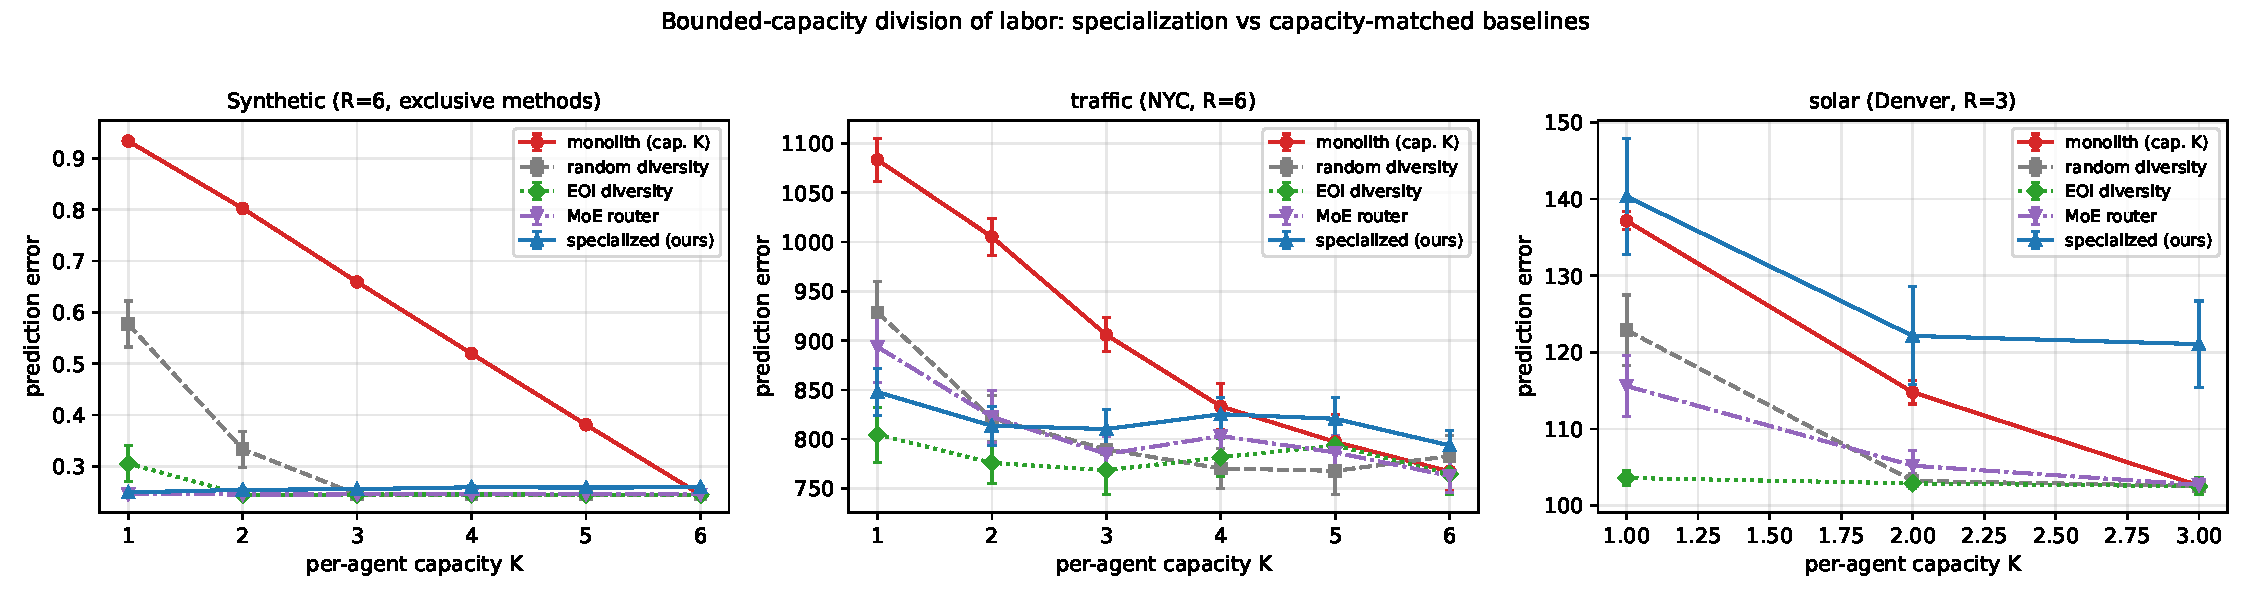
\includegraphics[width=\textwidth]{figures/fig6_capacity_division.pdf}
\caption{Coverage under bounded capacity: task error versus per-agent capacity
$K$ for the five allocation arms (95\% CIs), on the synthetic regime-champion
stream and real traffic data. The specialized population dominates at tight
capacity; purpose-built baselines close the gap as $K$ grows---coverage is a
commodity, and competition's edge is parsimony.}
\label{fig:capacity}
\end{figure}

\subsection{Results on Retention Under Non-Stationarity}

Regimes cycle (a sliding window of $W{=}3$ of $R{=}6$ regimes is active per
epoch), so every regime goes dormant and reactivates. This is where the five
arms dissociate exactly as Principle~\ref{prin:ria} predicts
(Figure~\ref{fig:nonstat}):

\begin{table}[h]
\centering
\small
\begin{tabular}{lcc}
\toprule
\textbf{Arm ($K{=}1$, hard model)} & \textbf{Post-reactivation error} &
\textbf{Retains?} \\
\midrule
Monolith & $1.015$ & no \\
MoE router & $0.928$ & no \\
Random diversity & $0.603$ & partially (coverage gaps) \\
Learned diversity & $0.322$ & yes \\
GAUSE & $0.283$ & yes \\
\midrule
\textit{Oracle fixed (skyline)} & \textit{0.253} & \textit{yes (given labels)} \\
\bottomrule
\end{tabular}
\caption{Post-reactivation error at $K{=}1$ under the hard (LRU) capacity
model. The two reward-driven arms cluster at the top (forgetting); the
reward-independent arms retain---fixed random niches only partially, because at
$K{=}1$ they may leave a regime uncovered, while learned diversity and GAUSE
cover and retain in full. The italicized last row is the oracle fixed-assignment
\emph{skyline}: handed both the labels and a perfect covering permutation, it
needs no discovery and marks the irreducible floor ($0.253$, the noise level).
GAUSE comes within $0.030$ of this skyline at $K{=}1$ \emph{without being given
the assignment}, and is statistically indistinguishable from it by $K{=}3$
(detail in Section~\ref{sec:oracle}; oracle skyline in Figure~\ref{fig:nonstat}).}
\label{tab:retention}
\end{table}

The population beats the capacity-matched monolith by $+33\%$ overall and
$+71\%$ in the post-reactivation window ($p<10^{-36}$ at $K{=}3$), and the
router---which matched competition on spatial coverage---fails here decisively
($0.928$ vs.\ $0.283$ at $K{=}1$, $p\sim10^{-35}$; the gap stays significant
through $K{=}4$, $p<10^{-12}$), closing only as $K \to R$. The specialized
population is essentially flat in $K$: even $K{=}1$ agents collectively form a
complete persistent memory.

\begin{figure}[t]
\centering
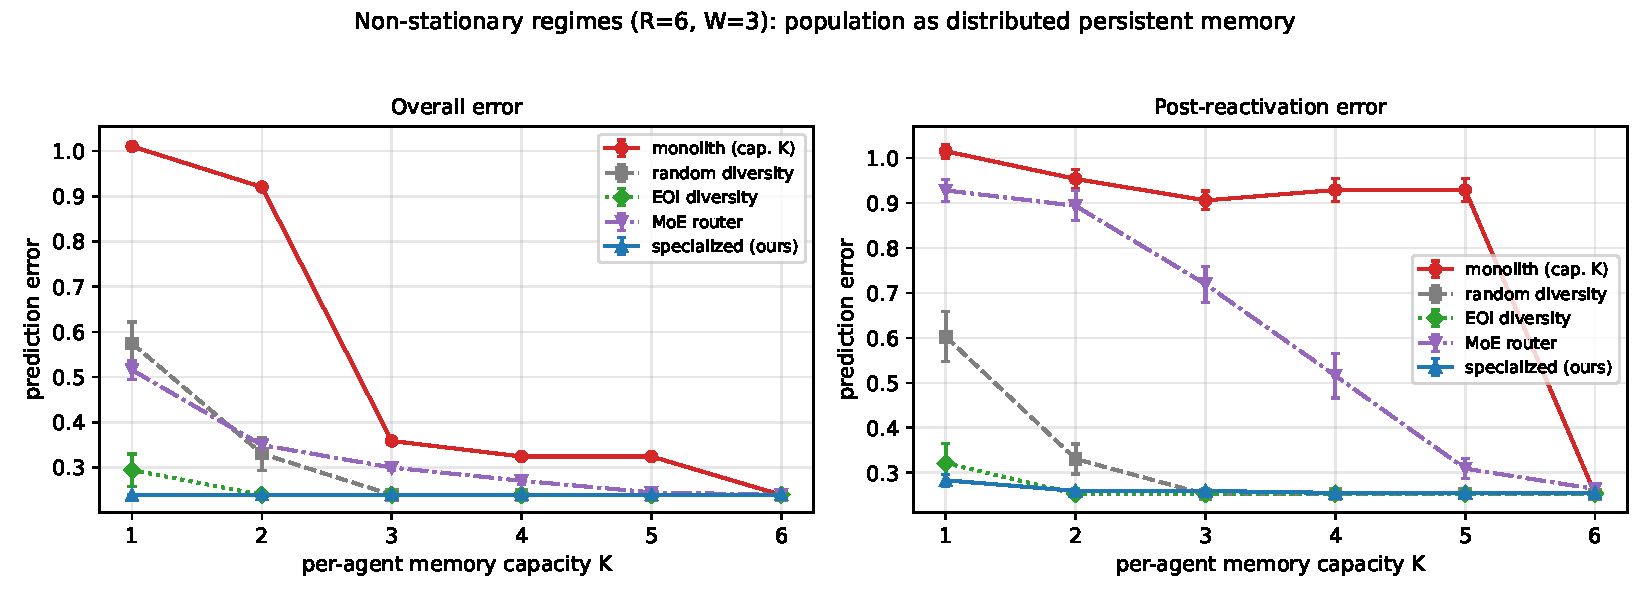
\includegraphics[width=\textwidth]{figures/fig7_nonstationary.pdf}
\caption{Retention under non-stationarity (hard LRU model, 95\% CIs): overall
and post-reactivation error versus capacity $K$ for the five mechanism arms plus
the oracle fixed-assignment \emph{skyline} (black dashed). The reward-driven arms
(monolith, MoE router) pay a persistent forgetting penalty that closes only as
$K \to R$; the reward-independent arms are flat in $K$ and track the oracle floor,
with GAUSE (blue) recovering the privileged skyline without being given the
assignment (Section~\ref{sec:oracle}).}
\label{fig:nonstat}
\end{figure}

\subsection{The Honest Competitor: an Oracle Fixed Assignment}
\label{sec:oracle}

A reader who has followed the setup will object that, since every arm is handed
the regime label $r_t$, the trivial baseline is not random diversity but an
\emph{oracle fixed assignment}: pin agent $i$ to a covering niche by hand---at
$K{=}1$ the identity permutation agent $i \mapsto$ regime $i$---with no learning of
\emph{where} to specialize. This arm is reward-independent and perfectly covering
\emph{by construction}, pays zero discovery cost, and so is the strongest possible
member of the retaining class. The natural question is then sharp: \emph{if I know
$R$ and the labels, why do I need emergent competition at all---why not just
hand-assign?}

We answer it directly by running the arm (the black dashed skyline in
Figure~\ref{fig:nonstat}). The oracle is
a \emph{skyline}, not a competitor: it cannot be beaten on retention because it
already has everything (labels, a perfect partition, no learning to do). The
result is that GAUSE \emph{matches it without the assignment}. At $K{=}1$ the
oracle floor is $0.253$ (the intrinsic noise level) and GAUSE reaches $0.283$---a
$0.030$ gap that is the measurable price of \emph{discovering} the covering
permutation from scratch rather than being told it. By $K{=}3$ the gap closes to
$0.006$ (GAUSE $0.260$ vs.\ oracle $0.254$), statistically indistinguishable
(Welch $p\approx0.05$), and both sit at the floor while the reward-driven arms are
still forgetting ($0.906$ and $0.719$). So the honest reading is: the value of
emergent competition is \emph{not} that it beats hand-assignment given the
labels---it cannot---but that it (i) recovers essentially all of the oracle's
retention automatically, with no pre-commitment to a partition, and (ii) degrades
gracefully off the $N\approx R$ diagonal where a hand-designed permutation is no
longer available (Section~\ref{sec:closing}). Competition buys you the oracle's
assignment when you are unwilling or unable to design it yourself; the latent-regime
result (Section~\ref{sec:latent}) is what lets it do so without the label too.
The GAUSE$\approx$oracle match is also not an artifact of the eviction rule: under
the soft interference model the two are indistinguishable at \emph{every} $K$
(differences $\le0.002$, $p>0.13$; at $K{=}1$, oracle $0.253$ vs.\ GAUSE $0.254$),
even tighter than under hard LRU.

\subsection{Ablation: Robustness to the Memory Model}

To confirm the dissociation is not an artifact of discrete LRU eviction, we re-run
the entire sweep under the soft interference model (no eviction; graded decay).
The picture is unchanged---the monolith forgets, the population retains
($\approx 0.25$, a $+70\%$ gap, $p\sim10^{-40}$), and the reward-driven router
stays significantly worse than the population ($+36\%$ at $K{=}1$; $+16\%$ at
$K{=}3$), degrading more gracefully but never closing the gap until $K\to R$. Full
sweep and figure in Appendix~\ref{app:soft}; the separation is a property of
reward-driven allocation, not of any particular forgetting mechanism.

\subsection{Dropping the Oracle Label: Class-Incremental GAUSE}
\label{sec:latent}

Every result so far is task-incremental: each arm is handed the regime label
$r_t$. The deepest question a reviewer can ask is whether the central
retention claim survives when that label is removed---the genuinely hard
\emph{class-incremental} setting, where which regime is active must be inferred. We
test it directly. The key realization is that the label is not actually needed: in
this environment regime $r$ is signalled by method $r$ being best, and \emph{which
method an agent played is observable}. So we let each agent carry its niche
affinity over the \emph{method} space---a proxy for the latent regime---instead of
over regimes. An agent learns ``I am the $M_3$ specialist'' without ever being told
``this is regime $R_3$.'' Because winner-take-all selects on realized quality, the
agent whose specialty method matches the active regime wins: the winner \emph{is}
the implicit regime estimate, and the true regime is used only to score retention,
never to drive any arm.

The result (Figure~\ref{fig:latent}) is that the dissociation survives label
removal. Label-free GAUSE self-organizes against the \emph{hidden} regimes
(specialization index $0.75$, coverage $0.86$---imperfect, with occasional
collisions, which is the honest signature of unsupervised recovery) and retains:
its post-reactivation error is $0.38$ at $K{=}1$ and flat in $K$, versus $1.07$ for
a label-free capacity-bounded monolith that forgets ($+65\%$, the same separation
the labelled experiment shows). The price of dropping the label is real but
modest---$0.38$ label-free versus $0.283$ label-given---and far smaller than the
gap to the forgetting baseline. Reactivation is detected purely from input
similarity: when a dormant regime returns, its method works again and the intact
specialist wins, with no label and no change-point detector. This converts the
class-incremental extension from a promissory note into a demonstrated result, and
is the strongest evidence that retention is a property of reward-independent
self-organization rather than of privileged access to the regime identity.

\begin{figure}[t]
\centering
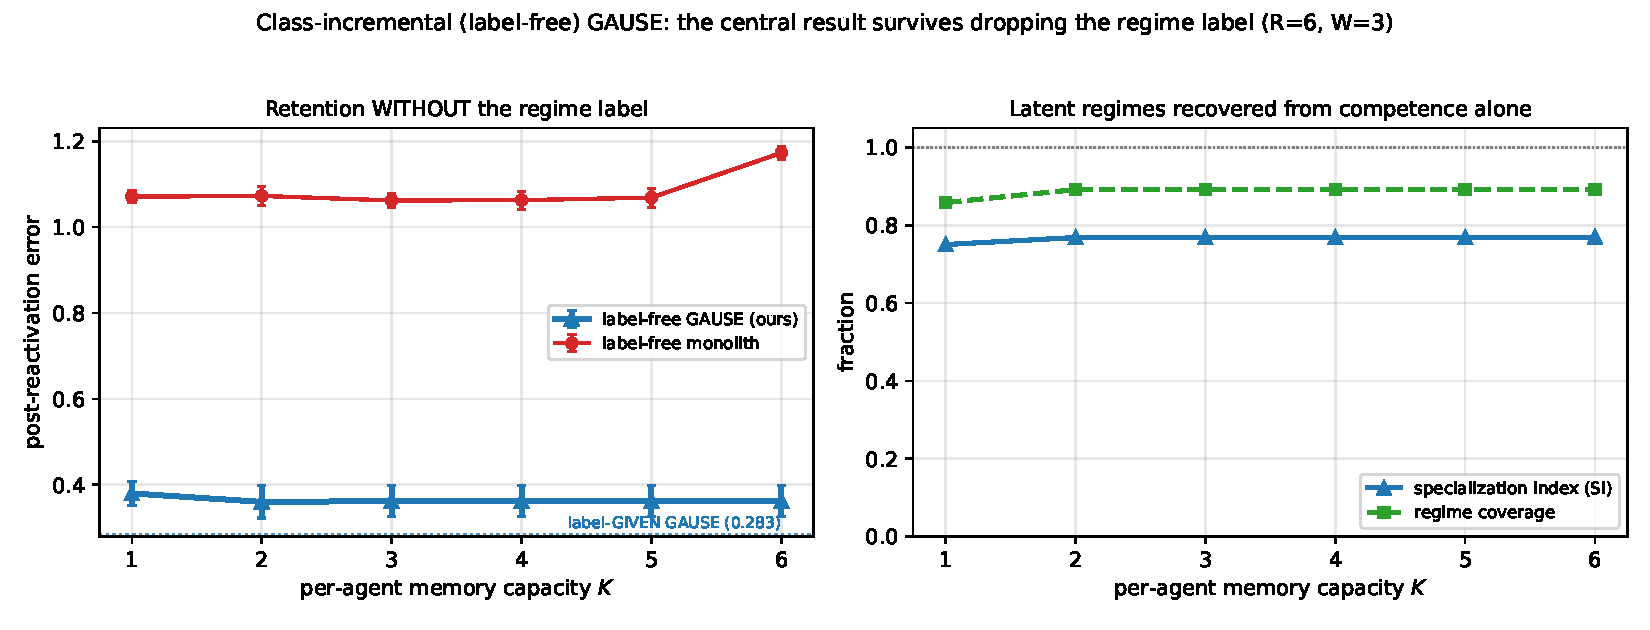
\includegraphics[width=\textwidth]{figures/fig14_latent_regime.pdf}
\caption{Class-incremental (label-free) GAUSE, with the regime label
\emph{removed} from every arm ($R{=}6$, $W{=}3$, hard LRU, 95\% CIs).
\textbf{Left:} post-reactivation error---label-free GAUSE ($\approx0.38$, flat in
$K$) retains while a label-free monolith forgets ($\approx1.07$); the dotted line
is the label-given GAUSE reference ($0.283$), the modest price of inference.
\textbf{Right:} the population recovers the latent regimes from competence alone
(specialization index $0.75$ and coverage $0.86$ at $K{=}1$, rising slightly with
$K$)---imperfect but clearly structured, the honest signature of unsupervised
partition discovery.}
\label{fig:latent}
\end{figure}

\emph{What this does and does not show (read this).} The method-space proxy is exact
\emph{by construction} here: in our synthetic stream regime $r$ is signalled by
method $r$ being uniquely best, a clean one-to-one correspondence, and the played
method is observable. So this experiment removes the \emph{label} but not the
assumption that a low-dimensional, observable signature separates the regimes---it
is honest class-incremental inference only to the extent that such a signature
exists. The part that must generalize is precisely this: on real, feature-rich data
with overlapping or non-identifiable methods the proxy is no longer exact, and
recovering the latent regimes becomes a genuine online clustering problem (the open
correspondence question of Section~\ref{sec:conclusion}). We therefore read
Figure~\ref{fig:latent} as a proof of concept that the competitive dynamics
\emph{can} self-supervise the partition when a separating signal is present, not as
evidence that they will on arbitrary inputs.

\subsection{Ablation: The Honest Audit}
\label{sec:audit}

Three controls scope all of the above. \textbf{(i)} SI is invariant to
regime-label shuffling: it measures organization, not structure. \textbf{(ii)}
An oracle structure-diagnostic shows four of six domains have a globally
dominant method (no exploitable regime structure); on the two structured domains
(traffic, solar), causal leakage-free regime labels beat shuffled labels by
$+15.4\%$ and $+12.8\%$. \textbf{(iii)} With \emph{unlimited} capacity, a single
regime-conditioned monolith matches or beats the population: division of labor
is a task-accuracy lever \emph{specifically} under bounded capacity and
non-stationarity, not in general. We consider this audit as much a contribution
as the positive results: it states exactly where the mechanism's value lives.

\subsection{Closing the Design Space: Function Approximation, a Hybrid Router,
Drift, and Population Sizing}
\label{sec:closing}

Four further experiments close the gaps a careful reader will press on: is the
router's failure an artifact of tabular learners, can a reward-driven router be
\emph{fixed}, what happens when a regime returns \emph{changed}, and what happens
when the population size leaves the $N\approx R$ diagonal?

\textbf{The router's forgetting is architecture-agnostic
(Figure~\ref{fig:funcapprox_ex}).} Replacing the tabular learners with
\emph{gradient-trained neural experts} (MLPs trained by SGD) on permuted-digits---a
standard continual-learning benchmark of $R{=}5$ pixel-permutation tasks, with the
number of experts $E$ as the capacity analog---reproduces the dissociation in full. At
$E{=}R$ the reward-driven MoE router's post-reactivation test error is $0.576$ versus
GAUSE's $0.218$ ($+62\%$ lower, $p\sim10^{-9}$), and the router does \emph{not} improve
with more experts (its still-learning gate keeps reallocating capacity to active tasks).
The forgetting is thus a property of reward-driven assignment, not of the tabular
substrate---the evidence the agentic-AI / MoE application narrative needs.

\textbf{The dissociation survives on a standard image benchmark
(Figure~\ref{fig:splitcifar}).} Because the gas-sensor reality check
(Section~\ref{sec:realdata}) showed the forgetting story belongs to the
representation-sharing regime rather than to linear-on-features, we put exactly that
surviving claim on a benchmark the continual-learning community recognizes:
\emph{Split-CIFAR-100} with small convolutional experts trained by SGD ($R{=}5$ disjoint
$10$-way tasks streamed through the same sliding-window recurrence schedule, so dormant
tasks genuinely reactivate). The dissociation reproduces: at $E{=}R$ GAUSE's
post-reactivation test error is $0.581$ versus the reward-driven router's $0.748$
($+22\%$ lower, $p\sim10^{-3}$), and---the diagnostic signature---GAUSE closes the gap
monotonically as capacity grows ($0.793\!\to\!0.581$ from $E{=}1$ to $E{=}R$) while the
router barely moves ($0.807\!\to\!0.748$) and the monolith is flat ($0.802$). The edge
is \emph{smaller} than on permuted-digits ($+22\%$ vs $+62\%$): on harder real images
with a small CNN and a short per-visit training budget, less is retained by anyone, so
there is less retention to dissociate---we report the attenuation rather than the
headline. The mechanism, however, transfers intact to a standard benchmark, which is
what the claim needed.

\textbf{A hybrid router with a reservation term
(Figure~\ref{fig:hybrid_ex}).} Keeping the reward-driven gate but adding an explicit
reservation---once the gate commits a regime to an expert, that expert pins the
regime's beliefs even while dormant---recovers most of the lost retention \emph{when
there is spare capacity}: at $K{=}3$ the post-reactivation error falls from the vanilla
router's $0.719$ to $0.374$ ($+48\%$, $p\sim10^{-11}$), approaching GAUSE ($0.260$). But
the fix \emph{cannot} help at $K{=}1$ ($0.928$, identical to vanilla): a single hard
slot cannot both serve the active regime and reserve a dormant one, whereas the
$N{=}R$ competitive population retains even at $K{=}1$ ($0.283$) by distributing memory
across idle specialists. Reward-\emph{independence of the protection} is the operative
property; competition obtains it for free, with no reservation bookkeeping and no
spare-capacity requirement.

\textbf{Intra-regime drift: when retention backfires
(Figure~\ref{fig:drift_ex}).} Finally we stress the win-only EG update directly: we let
each regime's optimal method \emph{drift} on every reactivation. Standard GAUSE pays for
its stability---a converged specialist holds its niche by identity and serves it with
stale beliefs, giving an overall error of $0.90$, \emph{worse} than a $K{=}3$ monolith
($0.35$) that is forced to relearn and stays current. This is the predicted ``stale
specialist'' failure, now quantified. A lightweight \emph{staleness trigger} (reset a
niche whose owner is confidently underperforming---drift, not noise---and soften its
affinity to re-open competition) recovers most of it ($0.43$ overall, $\sim53\%$ lower);
the residual post-drift penalty is the irreducible relearning cost. Reward-independent
retention is an asset under dormancy and a liability under drift, and a cheap trigger
restores adaptivity without sacrificing the dormancy benefit.

\begin{figure}[t]
\centering
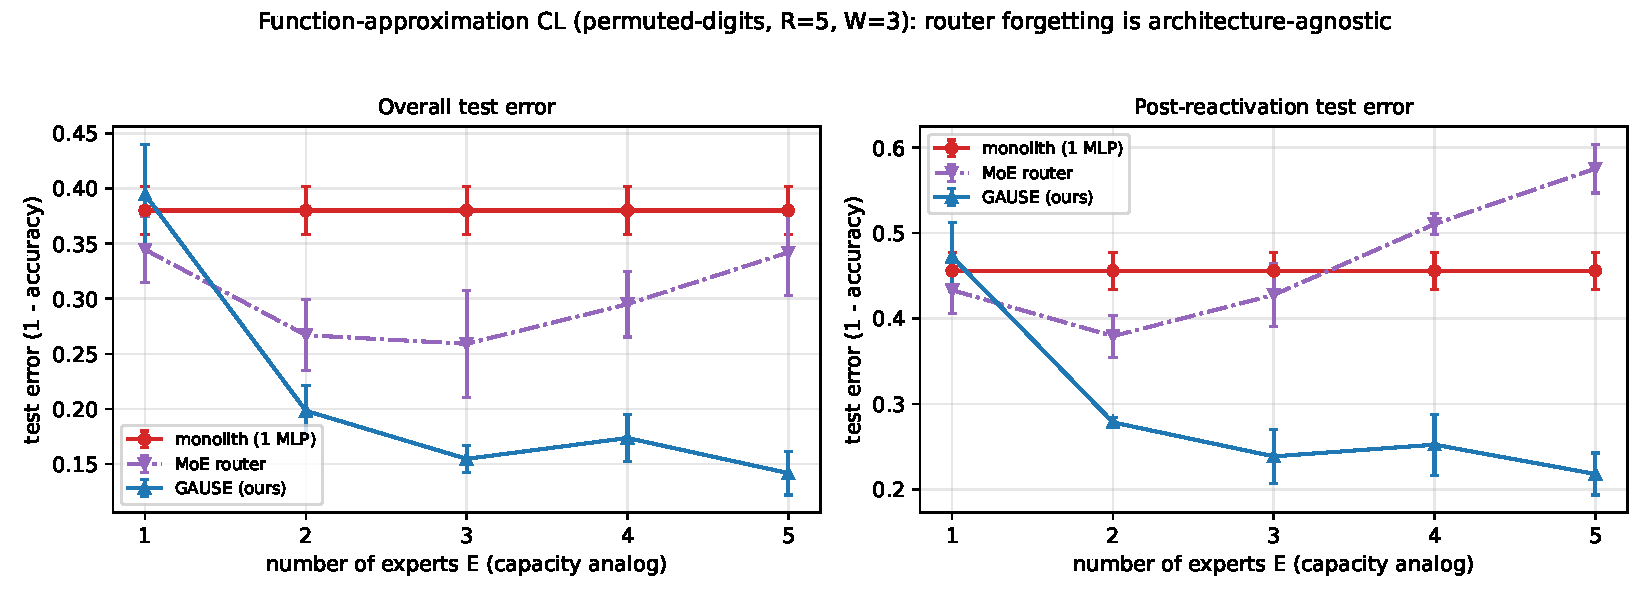
\includegraphics[width=\textwidth]{figures/fig11_function_approx_cl.pdf}
\caption{Function-approximation continual learning with gradient-trained MLP experts
(permuted-digits, $R{=}5$). The reward-driven router (purple) forgets dormant tasks and
does not improve with more experts $E$; GAUSE (blue) retains them ($+62\%$ lower
post-reactivation error at $E{=}R$). The router's failure is architecture-agnostic.}
\label{fig:funcapprox_ex}
\end{figure}

\begin{figure}[t]
\centering
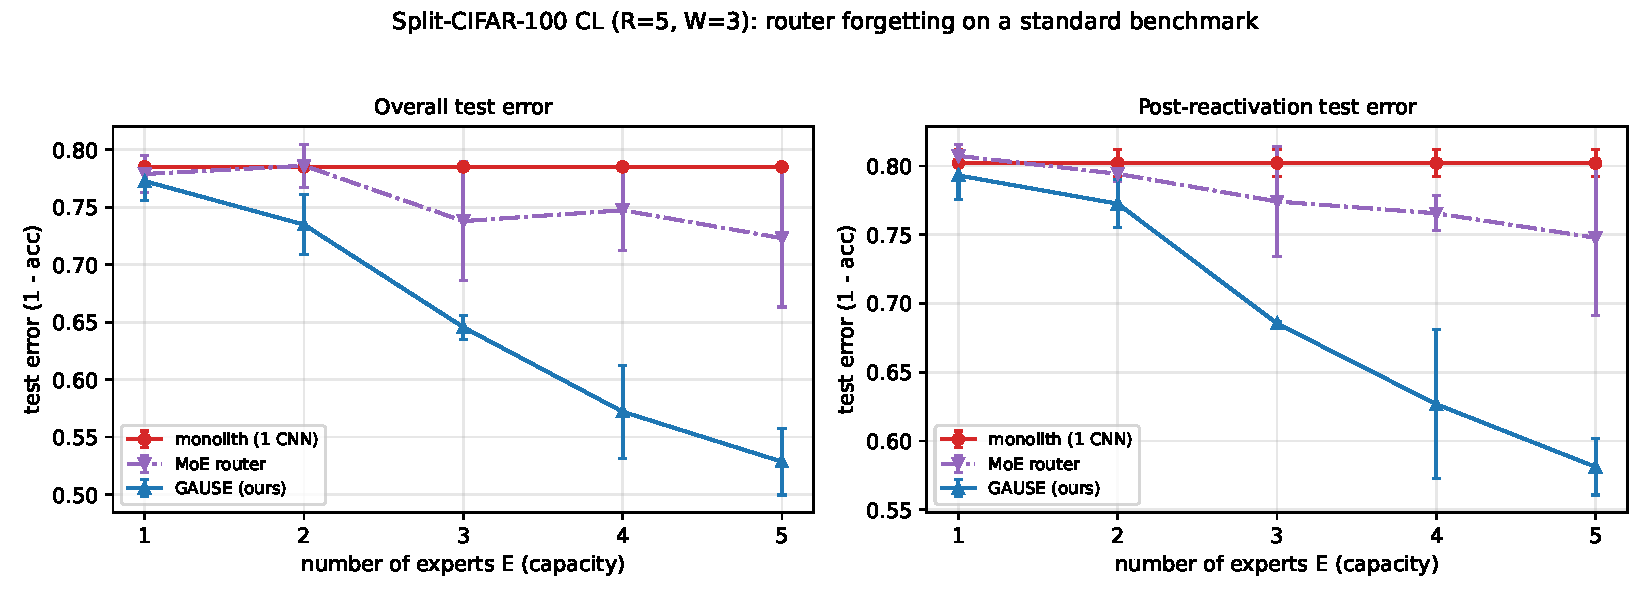
\includegraphics[width=\textwidth]{figures/fig_split_cifar_cl.pdf}
\caption{Split-CIFAR-100 with gradient-trained CNN experts ($R{=}5$ disjoint $10$-way
tasks, sliding-window recurrence, $4$ trials, $95\%$ CIs)---the surviving
representation-sharing claim on a standard benchmark. GAUSE (blue) lowers both overall
and post-reactivation test error monotonically as capacity $E$ grows; the reward-driven
router (purple) barely improves and the monolith (red) is flat. At $E{=}R$ GAUSE retains
$+22\%$ better than the router ($0.581$ vs $0.748$, $p\sim10^{-3}$)---a smaller but
significant edge than on the easier permuted-digits, honestly attenuated by the harder
images and short training budget.}
\label{fig:splitcifar}
\end{figure}

\begin{figure}[t]
\centering
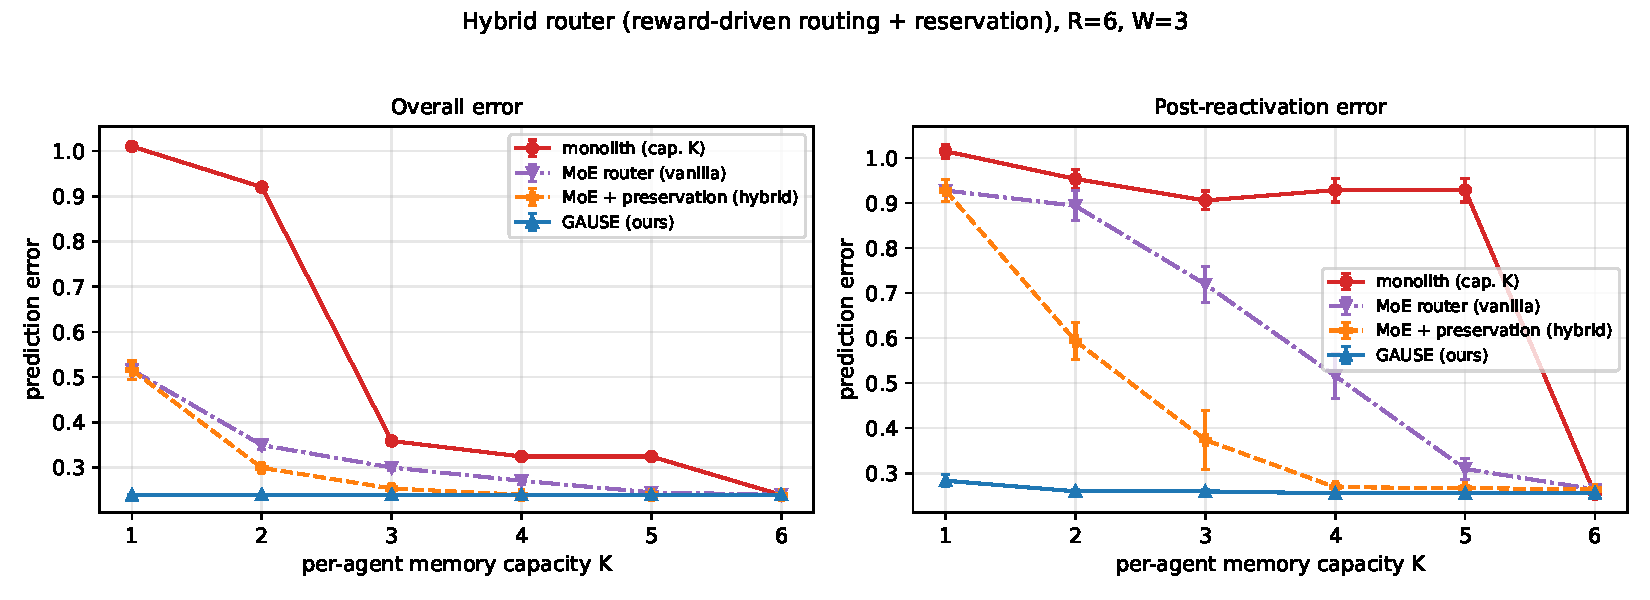
\includegraphics[width=\textwidth]{figures/fig9_hybrid_router.pdf}
\caption{Hybrid arm: reward-driven routing \emph{plus} a reservation term. It recovers
most retention with spare capacity ($+48\%$ at $K{=}3$) but cannot help at $K{=}1$;
the competitive population retains even at $K{=}1$. Reward-independence of protection
is the operative property.}
\label{fig:hybrid_ex}
\end{figure}

\begin{figure}[t]
\centering
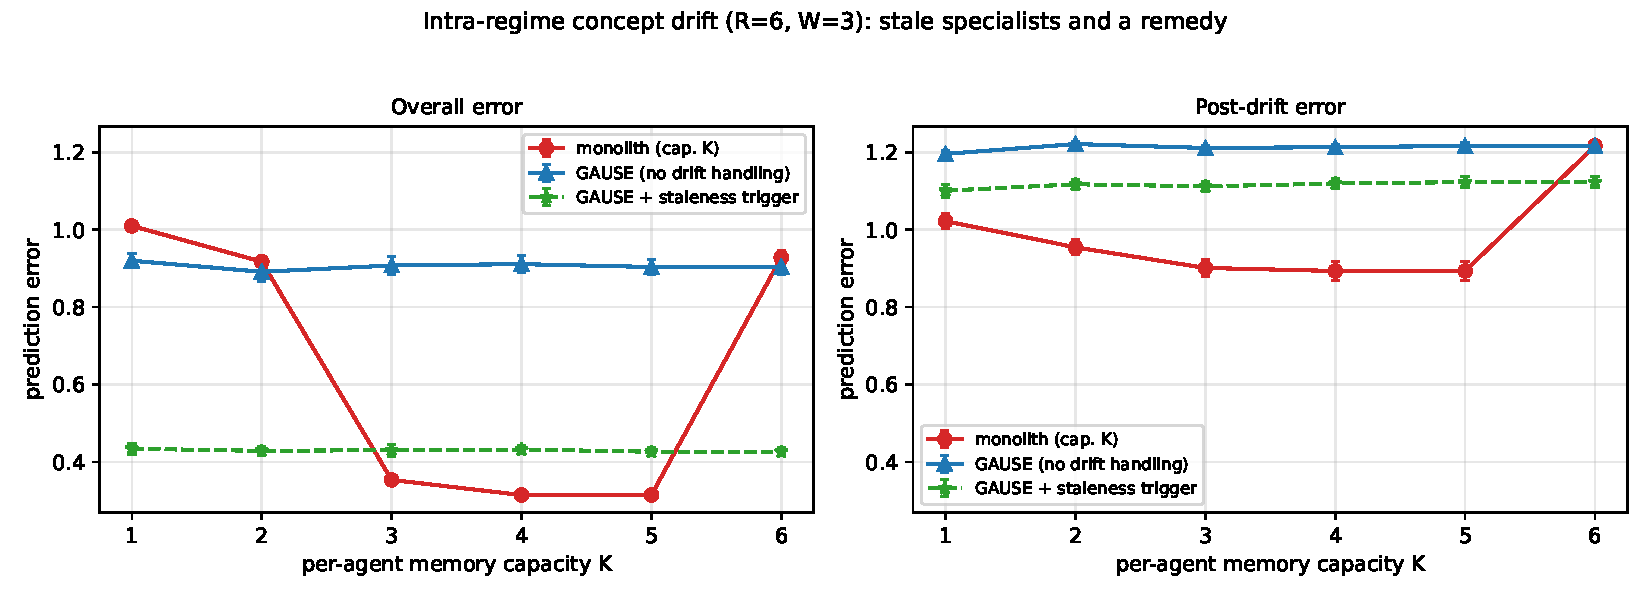
\includegraphics[width=\textwidth]{figures/fig10_intra_regime_drift.pdf}
\caption{Intra-regime concept drift. Standard GAUSE (blue) pins a stale specialist
(overall error $0.90$, worse than a relearning monolith); a staleness trigger (green)
recovers most of it ($0.43$). Reward-independent retention helps under dormancy and
hurts under drift.}
\label{fig:drift_ex}
\end{figure}

\textbf{Population sizing off the $N\approx R$ diagonal.} Sweeping $N$ on the
retention protocol characterizes both off-diagonal regimes (full sweep and figure in
Appendix~\ref{app:popsize}). The deployment-relevant summary: with \emph{scarce}
agents ($N<R$) coverage is governed by $N$, not by total capacity $N\!\cdot\!K$
(winner-take-all gives each agent one primary niche, so a larger $K$ does \emph{not}
rescue coverage); with \emph{abundant} agents ($N\gg R$) coverage saturates and
exactly $N-R$ agents idle harmlessly. The rule is therefore \emph{provision
$N\gtrsim R$}---surplus is harmless, deficit forgets.

\subsection{Real Data: The Class-Incremental Claim, Tested and Bounded
(UCI Gas Sensor Array Drift)}
\label{sec:realdata}

The class-incremental subsection above flagged the one assumption its synthetic
result could not shed: that a low-dimensional, observable signature separates the
regimes. We now test that assumption on real data---the UCI Gas Sensor Array Drift
dataset (13{,}910 samples, $128$ real sensor features, $6$ gas classes, $10$ batches
collected over $36$ months of genuine sensor drift, with \emph{no} method$\leftrightarrow$regime
bijection). We stream the batches in time order under the same sliding-window
dormancy schedule and measure post-reactivation accuracy
(Figure~\ref{fig:realdata}). The outcome is a clean, honest split---one claim holds,
one is bounded, one is refuted in this regime---and we report all three, because the
split is more informative than any single headline.

\textbf{(1) Full-capacity linear continual learning does \emph{not} forget here.}
A plain online multinomial-logistic classifier trained by naive SGD reaches
post-reactivation accuracy $0.68$ and overall accuracy $0.93$; experience replay is
identical; EWC is \emph{worse} ($0.44$), because its Fisher anchor fights the real
drift it should be adapting to. On these real, near-linearly-separable sensor
features there is simply nothing to catastrophically forget, so there is no
linear-on-features retention win to claim. The forgetting dissociation the framework
\emph{does} own lives one level up, in the representation-sharing regime: the
permuted-digits experiment (Figure~\ref{fig:funcapprox_ex}) shows the reward-driven
router forgetting ($+62\%$) with \emph{gradient-trained} experts, where learned
representations genuinely interfere, and the same dissociation reproduces on
\emph{Split-CIFAR-100} with convolutional experts ($+22\%$ at $E{=}R$,
$p\sim10^{-3}$; Figure~\ref{fig:splitcifar})---a standard benchmark, so the claim is
not an artifact of one toy dataset. Real data thus relocate---rather than
refute---the catastrophic-forgetting claim: it is a property of capacity-bounded
\emph{representation sharing}, not of arbitrary feature streams.

\textbf{(2) Label-free recovery collapses under real overlap.} Strip the label and
let each agent infer the class from the $128$-d vector: GAUSE-LF post-reactivation
accuracy falls to $0.00$, with specialization index $0.53$ and coverage $0.83$
(five of six classes ever owned). Critically, the label-free \emph{monolith} also
scores $0.00$---the ``GAUSE retains, monolith forgets'' dissociation that the
synthetic $1{:}1$ signature produced \emph{vanishes}. The mechanism is visible in
the traces: when a dormant class returns, its drifted features are nearest to a
\emph{currently active} class's prototype, so the implicit class estimate is simply
wrong. The method$\leftrightarrow$regime proxy was load-bearing after all. This
refutes the strong reading of the label-free headline on real overlapping drift and
confirms---rather than weakens---the scope we stated in
Section~\ref{sec:latent}: class-incremental GAUSE is a proof of concept for
\emph{separable-signal} regimes, not for arbitrary high-dimensional inputs.

\textbf{(3) Robustness, honestly inverted.} On the benign synthetic surrogate the
supervised baselines sit flat at $1.00$ (nothing to forget), so that sweep is
uninformative. On real drift the sweep \emph{is} informative, but not in GAUSE's
favor: replay is flat at $0.68$ across buffer sizes; EWC degrades monotonically as
its anchor tightens ($0.68$ at $\lambda{=}0$, through $0.44$ at $\lambda{=}20$, into
numerical divergence by $\lambda{=}300$); and GAUSE-LF is flat at $0.00$. The only
robustness point that survives is narrow and real---EWC's single knob can actively
hurt and must be kept near zero on a drifting stream, whereas competition has no
such knob---but here GAUSE's flat line sits \emph{below} the competitors, not above.

\textbf{What this does to the contribution.} Taken together the real data move the
paper off the performance axis. On a genuine recurring-regime stream the
parsimony-\emph{as-performance} reading does not hold: a one-line classifier with
labels beats label-free GAUSE outright, and full-capacity continual learning does
not forget. What survives contact with real data is the \emph{mechanism}: (i) the
reward-independence principle and its router-forgetting prediction, confirmed with
gradient-trained experts where representations actually interfere; and (ii) the
honest map of \emph{where} competition helps---bounded capacity, representation
interference, and separable regime signals---and where it does not. We therefore
read GAUSE as a mechanism/lens contribution rather than a benchmark winner, and have
aligned the abstract and the limitations accordingly.

\begin{figure}[t]
\centering
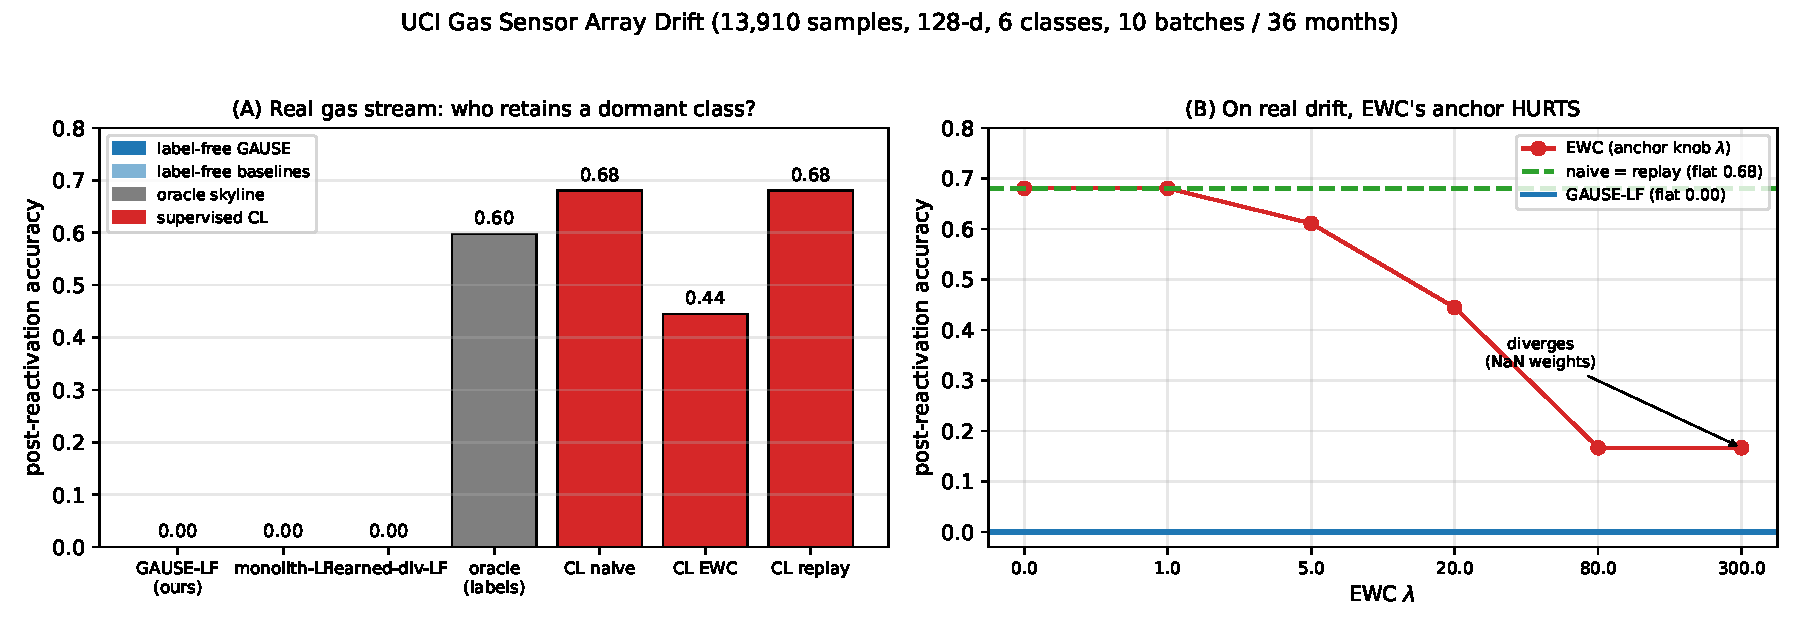
\includegraphics[width=\textwidth]{figures/fig_real_data_gas.pdf}
\caption{Real data (UCI Gas Sensor Array Drift). \textbf{(A)} Post-reactivation
accuracy by arm. All label-free arms---GAUSE included---collapse to $0$: a dormant
class's drifted features are routed to an active class's prototype, so the
dissociation against the label-free monolith \emph{disappears}. A full-capacity
supervised linear classifier (naive/replay) does not forget ($0.68$); EWC's anchor
hurts under drift ($0.44$). \textbf{(B)} The EWC $\lambda$ sweep on real drift:
anchoring monotonically degrades retention and eventually diverges---the opposite of
its flat $1.00$ on the benign surrogate. The honest reading: on real
near-linearly-separable features there is nothing to forget, so the
catastrophic-forgetting claim belongs to the representation-sharing neural regime
(Figure~\ref{fig:funcapprox_ex}), and the label-free claim is bounded to
separable-signal regimes.}
\label{fig:realdata}
\end{figure}

%==============================================================================
\section{Potential Applications}
\label{sec:applications}
%==============================================================================

GAUSE is a mechanism, not a model: it applies wherever (i) the
environment decomposes into recurring regimes, (ii) per-learner capacity is
bounded, and (iii) regimes go dormant and return. Those three conditions are
remarkably common. This section surveys the application domains where we
believe the mechanism---and especially its retention guarantee---has the most
leverage. Table~\ref{tab:apps} summarizes the mapping; a deployment recipe
follows at the end of the section.

\noindent\textbf{Evidence status (read this first).} The discussion below is
\emph{prospective}, and we are explicit about how far our evidence reaches. Two
domains---\emph{quantitative finance} (crypto, commodities) and \emph{distributed
sensing} (solar, weather, air quality)---use data drawn from the same families as
our validation domains, so the self-organization and bounded-capacity results
transfer most directly there. The agentic-AI / MoE memory case sits one tier below:
our function-approximation experiment (Section~\ref{sec:closing}) shows the router's
forgetting and GAUSE's retention with \emph{gradient-trained neural experts} on a
standard continual-learning benchmark, so the mechanism-level prediction is no longer
an analogy---but we have not deployed it inside a production-scale MoE or agent
framework, so the systems claim remains untested. The remaining domains (robot
fleets, cloud serving, clinical monitoring) are \emph{conjectures}: they satisfy the
three structural conditions on paper, but we have run no experiments in them. We
present the full survey because the mechanism's preconditions are domain-agnostic,
but the reader should treat everything past the first two subsections as a research
agenda, with the MoE case the only one backed by direct mechanism-level evidence.

\begin{table}[h]
\centering
\small
\begin{tabular}{p{3.0cm} p{3.1cm} p{3.1cm} p{4.4cm}}
\toprule
\textbf{Field} & \textbf{Regimes} & \textbf{Learners} &
\textbf{Dormancy risk (what is forgotten)} \\
\midrule
Agentic AI memory & task/skill families & skill modules, expert pools &
rarely-invoked skills overwritten by frequent ones \\
Quantitative finance & market regimes (trend, crisis, range) &
strategy pool / capital sleeves & crisis playbooks decay during calm
markets \\
Edge sensing \& IoT & seasonal/diurnal patterns, fault modes &
on-device models & rare fault signatures lost between
occurrences \\
Robot fleets & zones, task types, failure modes & robots / controllers &
seldom-used manipulation skills degrade \\
Cloud serving & workload classes & autoscaled worker pools &
warm capacity for bursty rare workloads \\
Clinical monitoring & patient subpopulations, rare conditions &
model ensemble & rare-condition detectors drowned by common cases \\
\bottomrule
\end{tabular}
\caption{Mapping GAUSE onto application domains. In every row the
dormancy column is the failure a reward-driven (usage-driven, profit-driven,
traffic-driven) allocator suffers and a reward-independent population
structurally avoids.}
\label{tab:apps}
\end{table}

\subsection{Quantitative Finance: Regime-Switching Strategy Pools}

Financial markets are the canonical regime-switching environment---trending,
mean-reverting, high-volatility, and crisis regimes recur on irregular
schedules \cite{kirilenko2017flash}---and two of our six validation domains
(crypto, commodities) are financial. The standard industry practice is
reward-chasing by construction: capital and research attention flow to the
strategies that performed recently, and strategies that lose relevance are
retired. Our results identify the precise cost of that practice. A crisis
regime may be dormant for years; a capital allocator driven by recent P\&L
(the financial analogue of a learned gate) starves the crisis specialists,
their infrastructure and calibration decay, and when the regime reactivates
the desk pays the full relearning cost---at the worst possible time. A
GAUSE-style strategy pool inverts this: strategies compete for
regimes, the winner-take-all dynamics assign each strategy a niche, and
converged specialists are \emph{retained through dormancy by identity}, not
by P\&L. The niche bonus $\lambda$ has a natural reading as a diversification
mandate, and the capacity bound $K$ models the real constraint that a single
desk cannot stay calibrated to every market state. Three concrete uses:
(i) a \textbf{regime-specialist ensemble} for return forecasting, where the
dormant-regime specialist (e.g., the short-volatility-crash model) is kept
warm; (ii) \textbf{market-making parameter banks}, where quoting profiles
specialized to liquidity regimes are retained across regime cycles; and
(iii) \textbf{risk-model committees}, where stress-period models must survive
long calm stretches---exactly the retention property reward-driven model
selection lacks.

\subsection{Distributed Sensing and Edge Intelligence}

Sensor networks and edge deployments are populations of capacity-limited
learners by physical necessity: each device has tight memory and compute, and
the environment it models has strong seasonal and episodic structure (diurnal
cycles, weather patterns, rare fault signatures). Centralized coordination is
expensive precisely where edge deployment is attractive. GAUSE needs
only a local competition signal (which device best predicted the current
window), so a fleet can partition pattern-space without a coordinator: some
devices become storm specialists, others baseline-drift specialists. The
retention property matters most for \textbf{rare-event detection}: a fault
signature seen once a year is a dormant regime, and a usage-driven model
update schedule will overwrite it. Our solar, weather, and air-quality domains
are direct evidence that the mechanism organizes correctly on exactly this
kind of data.

\subsection{Other Candidate Domains}

The remaining domains in Table~\ref{tab:apps} share the same three
preconditions but we have run no experiments in them; we keep them brief and
explicitly conjectural. \textbf{Agentic-AI / MoE memory} is the case our theory
engages most directly: agent skill libraries and MoE expert pools both face
bounded capacity and a long tail of rarely-invoked competences, and any
recency- or utility-driven eviction (LRU caches, usage-weighted distillation,
gates trained on task loss) is a reward-chasing allocator that
Principle~\ref{prin:ria} predicts will overwrite the skill needed \emph{next
quarter} because it emits no usage signal \emph{today}; letting experts compete
and then pinning the converged assignment realizes the gate-freezing
prescription of MoE continual-learning theory \cite{li2024moecl} without a
freeze schedule. This case is backed by our function-approximation
continual-learning experiments on two standard benchmarks (permuted-digits and
Split-CIFAR-100; Section~\ref{sec:closing}), the evidence here that goes beyond analogy. \textbf{Multi-robot fleets}
(zones/task-types as regimes; battery, gripper, and local-map budgets as
capacity) could partition a floor through win-driven affinity with no message
passing, keeping seldom-used skills warm. \textbf{Cloud serving} maps cleanly
onto our arms---autoscaling is the monolith, a learned request router is the MoE
arm, static over-provisioning is random diversity---and a competitive worker
pool would pin warm specialists for bursty rare workload classes against the
cold-start penalty. \textbf{Clinical monitoring} treats patient subpopulations
or rare conditions as regimes, dedicating ensemble members to rare presentations
that aggregate-performance updates would otherwise drown out. In all four, the
structure diagnostic (Section~\ref{sec:audit}) is the prerequisite test: if one
model dominates everywhere, the population adds nothing.

\subsection{When Not to Use It}

The audit section is a user manual in miniature, and we restate it as
deployment guidance. GAUSE does \emph{not} pay when: (i) capacity is
effectively unlimited---a single regime-conditioned model then matches the
population with less machinery; (ii) the environment has no regime structure
(one method dominates globally)---our oracle diagnostic detects this case in
advance; or (iii) regimes never go dormant---without non-stationarity,
retention is free and reward-driven routing is a fine choice. The mechanism's
value concentrates precisely where all three conditions bind, which the
applications above are selected to satisfy.

\noindent\textbf{Two failure modes the mechanism does not yet handle.} Beyond
those scope limits, the converged assignment has two known blind spots that a
deployer must weigh. \emph{(a) Within-niche drift.} The EG affinity update moves
identity only on \emph{wins} (positive evidence of fit), so a specialist does not
spontaneously relinquish a niche it is silently getting worse at: if a regime's optimal
method \emph{drifts} while the specialist idles, the converged assignment pins a stale
specialist in place. We now test this (Section~\ref{sec:closing},
Figure~\ref{fig:drift_ex}): under drift, standard GAUSE's overall error ($0.90$) is
\emph{worse} than a relearning monolith's ($0.35$), and a lightweight staleness trigger
that re-opens competition recovers most of it ($0.43$). The remedy works but leaves a
residual relearning cost, and we have not characterized drift rate or detection
threshold in general---so drift remains a deployment risk to weigh. \emph{(b)
Off-diagonal population sizing.} Our clean one-per-regime equilibrium and coverage
guarantee are \emph{proved} for $N \approx R$; the off-diagonal behavior we now
\emph{measure} (Section~\ref{sec:closing}, Figure~\ref{fig:popsize_ex}). Scarce agents
($N<R$) leave regimes uncovered---and crucially, coverage tracks $N$ rather than total
capacity $N\!\cdot\!K$, so a bigger per-agent budget does not help---while abundant
agents ($N\gg R$) idle harmlessly. The remaining gap is theoretical (no proof of the
off-diagonal equilibrium) and mechanistic (letting scarce agents fill $K>1$ slots).

\begin{designbox}
\textbf{Deployment recipe.} (1) Define regimes: a discrete, recurring
partition of the input stream (volatility bands, workload classes, seasonal
modes). (2) Define the quality signal: any per-step scalar comparable across
learners. (3) Set capacity $K$ honestly: how many regimes can one learner
stay calibrated on? (4) Run winner-take-all competition with the EG affinity
update ($\eta \approx 0.6$, $\lambda \in [0.2, 0.4]$ or $0$ for the pure
mechanism). (5) Read out the converged assignment and \emph{pin it}: the
assignment, not the gate, decides who holds what. (6) Re-open competition only
when the regime inventory itself changes.
\end{designbox}

\noindent\textbf{Honest accounting of what ``no machinery'' means.} We claim
competition needs no gate, no freezing schedule, and no diversity coefficient, and
that is true---but the recipe makes clear that effort is \emph{relocated}, not
eliminated. Steps (1)--(3) still demand the practitioner supply a discrete regime
partition, a cross-learner-comparable quality signal, and a capacity budget $K$;
these are real design decisions, and on a novel domain the regime partition can be as
hard to get right as a gate. Step (6) is, in particular, a \emph{freeze trigger}:
pinning the assignment until the regime inventory changes is exactly a freeze, except
that the condition is ``inventory changed'' rather than ``step count exceeded.''
Competition's genuine advantage is that the freeze happens \emph{automatically and at
the right time} (when competition converges) rather than on a schedule the
practitioner must tune---not that the notion of freezing has disappeared.

%==============================================================================
\section{Conclusion and Future Work}
\label{sec:conclusion}
%==============================================================================

We presented GAUSE, a minimal framework in which winner-take-all
competition over a niche-affinity simplex makes a population of capacity-bounded
learners self-organize into one-per-regime specialists---with no communication,
shared rewards, gates, or diversity objectives. The framework's deepest property
is that its converged assignment is \emph{reward-independent}: specialists hold
niches by identity, idle through dormancy, and thereby retain what reward-driven
allocators---including the standard learned MoE router---systematically forget.
Across five capacity-allocation mechanisms, retention tracks
reward-independence of assignment five-for-five, and an oracle fixed-assignment
skyline---handed both the labels and a perfect covering permutation---confirms the
ceiling: GAUSE recovers it to within $0.030$ at $K{=}1$ and indistinguishably for
$K\ge3$ without being given the assignment. Across six real-world domains
and controlled synthetic tasks, competition matches purpose-built diversity and
routing baselines on spatial coverage with none of their machinery, and
separates from them decisively on retention ($0.283$ vs.\ the router's $0.928$ at
$K{=}1$, $\sim$70\% lower, $p\sim10^{-35}$, robust to the memory model). An honest audit bounds the claim:
with slack capacity and stationary regimes, a regime-conditioned monolith
suffices; division of labor pays specifically when capacity binds and the world
shifts.

Section~\ref{sec:closing} closes four of the gaps this document is explicit about.
\textbf{(i)} A function-approximation demonstration confirms the router's failure is
architecture-agnostic on \emph{two} standard benchmarks: with gradient-trained MLP
experts on permuted-digits ($+62\%$) and convolutional experts on Split-CIFAR-100
($+22\%$, $p\sim10^{-3}$), the reward-driven router forgets while GAUSE retains at
$E{=}R$, converting the central prediction---and the agentic-AI/MoE application
story---from analogy into evidence. \textbf{(ii)} A hybrid allocator (a reward-driven
router \emph{plus} a reservation term) recovers most of the lost retention when spare
capacity exists but not at $K{=}1$, confirming that reward-\emph{independence of
protection} is the operative property and that competition obtains it for free.
\textbf{(iii)} An intra-regime drift experiment quantifies the stale-specialist risk
(standard GAUSE worse than a relearning monolith under drift) and shows a lightweight
staleness trigger recovers most of it. \textbf{(iv)} A population-sizing sweep
characterizes both sides of the $N\approx R$ diagonal: surplus agents idle harmlessly,
while scarce agents under-cover in proportion to $N$ (not $N\!\cdot\!K$), yielding the
deployment rule \emph{provision $N\gtrsim R$}.

A real-data test on the UCI Gas Sensor Array Drift stream
(Section~\ref{sec:realdata}) bounds the headline honestly: on near-linearly-separable
real features a full-capacity online classifier does \emph{not} catastrophically
forget, so the retention dissociation is a property of the representation-sharing
regime---confirmed by the two neural benchmarks above---rather than of arbitrary
feature streams, and the label-free recovery collapses under real overlap. On real
data, accordingly, the contribution is a \emph{mechanism and lens}, not a performance
win---which we regard as the more durable claim.

Several directions remain. \textbf{First}, drift handling beyond our trigger:
characterizing drift rate, detection threshold, and the dormancy--drift interaction,
since a residual relearning cost remains. \textbf{Second}, the \emph{theory} of
off-diagonal population sizing: we now measure that scarce agents ($N<R$) under-cover
(coverage tracks $N$, not $N\!\cdot\!K$) and abundant agents ($N\gg R$) idle harmlessly
(Section~\ref{sec:closing}), but a proof of the off-diagonal equilibrium, a mechanism
letting scarce agents exploit $K>1$, and scaling decentralized competition over hundreds
of regimes with churn and partial observability all remain open.
\textbf{Third}, removing the oracle regime label---which we now \emph{demonstrate}
rather than defer (Section~\ref{sec:latent}). Letting each agent carry its niche
affinity over the observable method space (a proxy for the latent regime) makes
GAUSE class-incremental: it self-organizes against the hidden regimes (SI $0.75$,
coverage $0.86$) and retains ($0.38$ post-reactivation at $K{=}1$ versus $1.07$ for
a label-free forgetting monolith), detecting reactivation purely from input
similarity. Tested on \emph{real}, feature-rich data with genuine overlap (UCI gas
sensor, Section~\ref{sec:realdata}), however, this label-free recovery
\emph{collapses} (post-reactivation $\to 0$): the synthetic
method$\leftrightarrow$regime signature was load-bearing, and the class-incremental
result is bounded to \emph{separable-signal} regimes. What remains open is therefore
the genuinely hard case the gas data expose---recovering latent regimes under
\emph{non-separable} real overlap---for which the correspondence between emergent
win-clusters and a stable latent labeling (online competitive-clustering / EM) is the
theoretical core.
\textbf{Finally}, deployment in the application domains of
Section~\ref{sec:applications}---trading-strategy pools, sensor networks, and expert
pools inside large models---where the parsimony of competition (an automatic,
correctly-timed freeze rather than a tuned schedule, and no diversity coefficient) is
most valuable.

%==============================================================================
\appendix
%==============================================================================

\section{Per-Domain Self-Organization}
\label{app:perdomain}

Figure~\ref{fig:crossdomain} reports the Specialization Index across all six
real-world domains (the summary cited in Section~\ref{sec:experiments}). We treat
this as a diagnostic, not a headline: SI certifies organization, not exploitable
structure (Section~\ref{sec:audit}).

\begin{figure}[h]
\centering
\includegraphics[width=0.78\textwidth]{figures/fig1_cross_domain_si.pdf}
\caption{Emergent self-organization across the six real-world domains:
GAUSE reaches SI $\approx 0.99$ everywhere, while homogeneous and random
baselines stay near zero.}
\label{fig:crossdomain}
\end{figure}

\section{Robustness: Soft (Interference) Memory Model}
\label{app:soft}

Re-running the entire non-stationary sweep under the soft interference model (no
eviction at all; every learning update on the active regime decays the
pseudo-counts of the agent's other held regimes) reproduces the dissociation
(Figure~\ref{fig:soft}): the monolith still forgets (post-reactivation error
$0.85$--$0.92$ at $K\le3$), the specialized population still retains ($\approx0.25$,
a $+70\%$ gap, $p\sim10^{-40}$), and the router remains significantly worse than the
population ($+36\%$ at $K{=}1$, $p\sim10^{-8}$; $+16\%$ at $K{=}3$). The router
degrades more gracefully under graded interference than under hard eviction but never
closes the gap until $K\to R$: the separation is a property of reward-driven
allocation, not of any particular forgetting mechanism.

\begin{figure}[h]
\centering
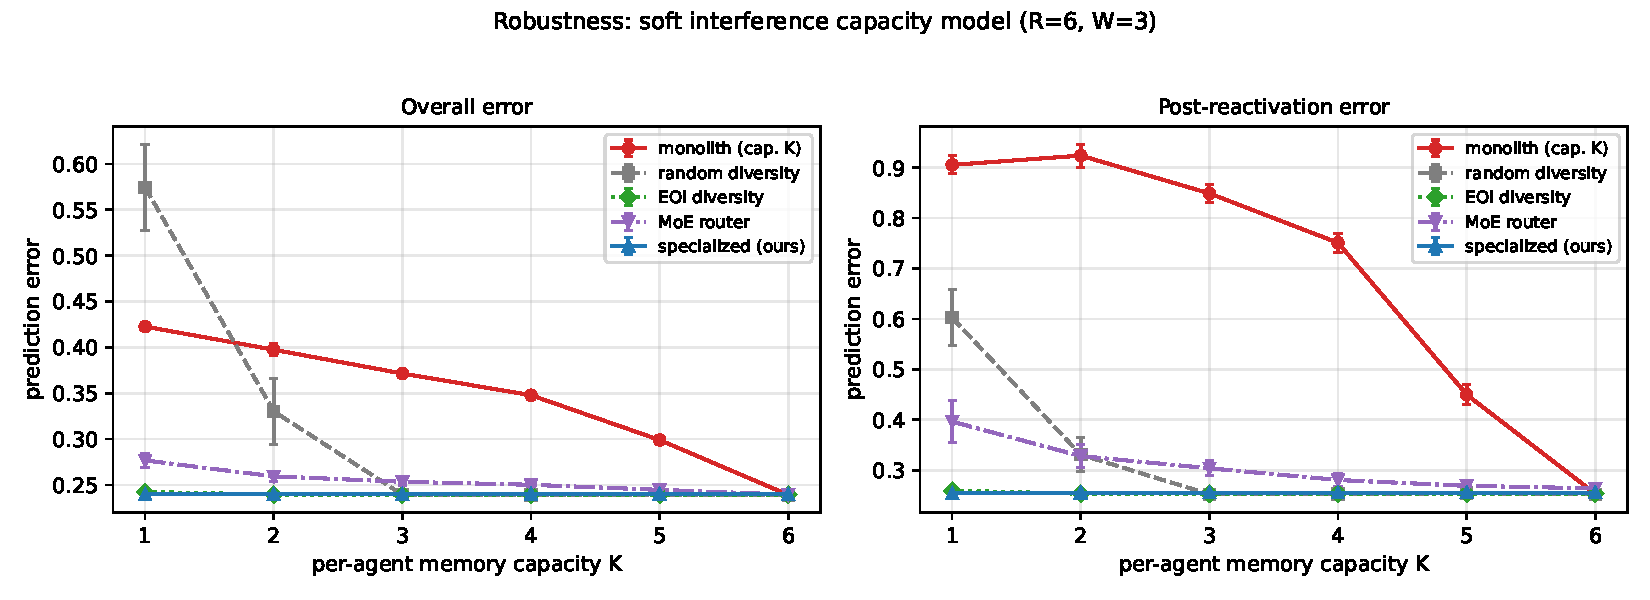
\includegraphics[width=\textwidth]{figures/fig8_nonstationary_soft.pdf}
\caption{Robustness to the capacity model: the full non-stationary sweep re-run
under the soft interference-decay model (no eviction). The reward-independence
dissociation survives intact, ruling out an artifact of discrete LRU eviction.}
\label{fig:soft}
\end{figure}

\section{Population Sizing Off the $N\approx R$ Diagonal}
\label{app:popsize}

Our equilibrium and coverage arguments assume $N\approx R$; sweeping $N$ on the
retention protocol ($R{=}6$) characterizes both off-diagonal regimes
(Figure~\ref{fig:popsize_ex}). With \emph{scarce} agents ($N<R$), coverage is capped
and governed by $N$, not by total capacity $N\!\cdot\!K$: winner-take-all gives each
agent one primary niche, so at $N{=}3$ coverage is only $\approx0.4$--$0.5$ and
post-reactivation error stays high \emph{even at $K{=}2$}, where total capacity would
in principle suffice---the spare slot goes unused. With \emph{abundant} agents
($N\gg R$) coverage saturates, exactly $N-R$ agents idle, and retention does not
regress. The deployment rule is therefore: provision $N\gtrsim R$ (surplus is
harmless, deficit forgets), and do not expect a larger $K$ to substitute for more
agents when agents are scarce.

\begin{figure}[h]
\centering
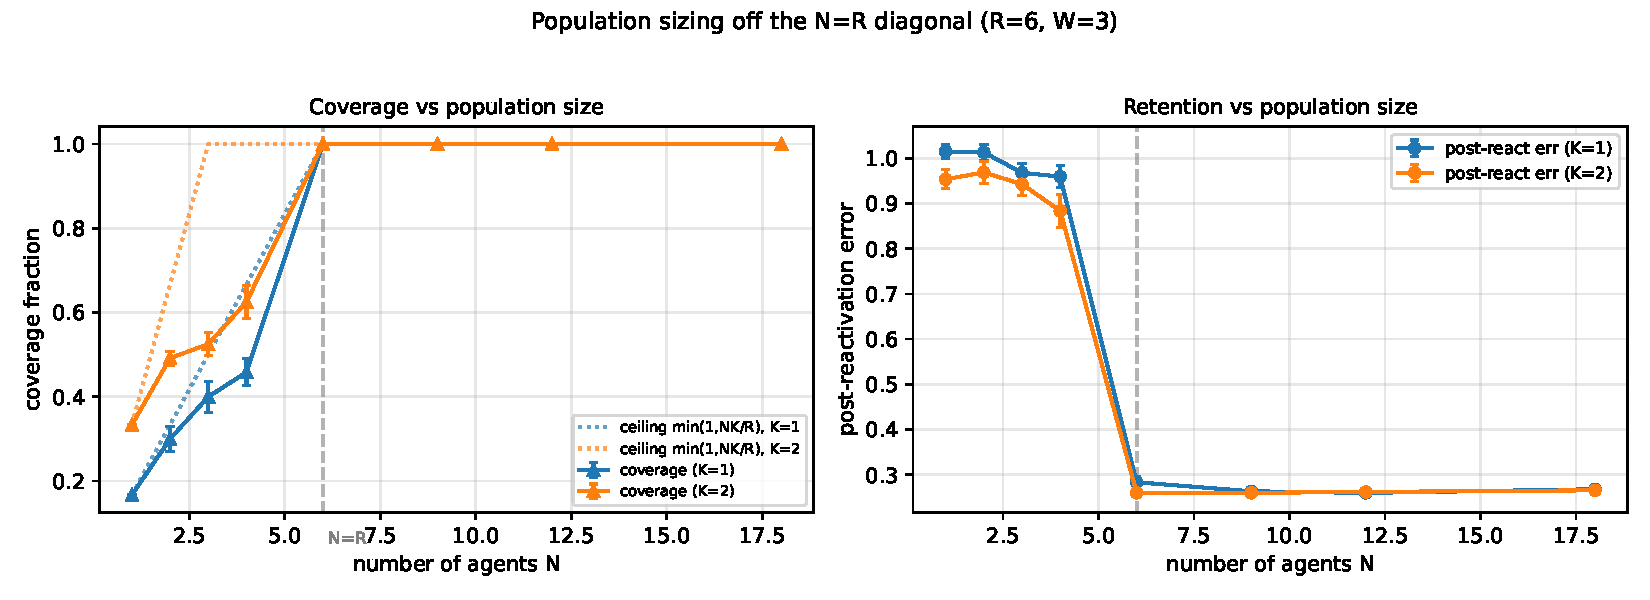
\includegraphics[width=\textwidth]{figures/fig12_population_sizing.pdf}
\caption{Population sizing off the $N\approx R$ diagonal ($R{=}6$). Below $N{=}R$,
coverage (left) tracks $N$ rather than the feasibility ceiling $\min(1,N\!K/R)$ and
retention (right) degrades; for $N\geq R$ coverage saturates and surplus agents idle
($N-R$ redundant) without harming retention.}
\label{fig:popsize_ex}
\end{figure}

\bibliographystyle{plain}
\bibliography{references}

\end{document}
